\documentclass[11pt]{amsart}

% Encoding and fonts
\usepackage[T1]{fontenc}
\usepackage[utf8]{inputenc}

% Math packages
\usepackage{amsmath}
\usepackage{amssymb}
\usepackage{amsfonts}
\usepackage{amsthm}
\usepackage{mathtools}

% Layout and utilities
\usepackage{geometry}
\usepackage{enumitem}
\usepackage{graphicx}
\usepackage{booktabs}
\usepackage{array}
\usepackage{xcolor}
\usepackage{listings}
\usepackage{mathrsfs}
\usepackage[hidelinks]{hyperref}

\geometry{margin=1in}

\numberwithin{equation}{section}
\setcounter{tocdepth}{3}
\setcounter{secnumdepth}{3}

% ---------------------------------------------------------
% Theorem-like environments
% ---------------------------------------------------------
\theoremstyle{plain}
\newtheorem{theorem}{Theorem}[section]
\newtheorem{proposition}[theorem]{Proposition}
\newtheorem{lemma}[theorem]{Lemma}
\newtheorem{corollary}[theorem]{Corollary}
\newtheorem{conjecture}[theorem]{Conjecture}

\theoremstyle{definition}
\newtheorem{definition}[theorem]{Definition}
\newtheorem{experiment}[theorem]{Experiment}
\newtheorem{heuristic}[theorem]{Heuristic}

\theoremstyle{remark}
\newtheorem{remark}[theorem]{Remark}

% ---------------------------------------------------------
% Macros
% ---------------------------------------------------------
\newcommand{\N}{\mathbb N}
\newcommand{\C}{\mathbb C}
\newcommand{\one}{\mathbf 1}
\newcommand{\epsfun}{\varepsilon}
\newcommand{\mob}{\mu}
\newcommand{\zetaR}{\zeta}
\newcommand{\Fsurf}{F}
\newcommand{\Vjump}{V}
\newcommand{\TauSum}{\mathcal T}
\newcommand{\Jordan}{\mathcal J}
\newcommand{\Mang}{\operatorname{Mang}}
\newcommand{\Sel}{\operatorname{Sel}}
\newcommand{\Neck}{\mathcal N}
\newcommand{\Div}{\operatorname{Div}}
\newcommand{\supp}{\operatorname{supp}}
\DeclareMathOperator{\rank}{rank}
\DeclareMathOperator{\tr}{tr}
\DeclareMathOperator{\diag}{diag}
\DeclareMathOperator{\Res}{Res}

\lstset{
  basicstyle=\ttfamily\scriptsize,
  breaklines=true,
  frame=single,
  columns=fullflexible,
  showstringspaces=false,
  language=Python
}

\title{A Divisibility Surface Built from the Moebius Function:\\Finite Inversion, Dirichlet Transforms, and Operator Questions}
\author{Victor Casana-Giner}
\date{August 2026}

\begin{document}
\pagestyle{plain}

\begin{abstract}
We study the two-parameter arithmetic surface
\begin{equation}
\Fsurf(n,r)=\sum_{\substack{a\mid n\\ a>r}}\mob(n/a),
\qquad n\ge 1,\quad r\ge 0.
\label{eq:abstract_F}
\end{equation}
The construction is elementary: it is a thresholded partial sum of the divisor-poset Moebius kernel.  The main rigorous content is a finite unimodular minor, its explicit inverse, a Frobenius-norm identity controlled by the divisor summatory function, and an exact intertwining identity between ordinary first differences and Dirichlet convolution.  We also record how the vertical jump field gives the classical quotient \(\zetaR(s+w)/\zetaR(s)\), how Jordan totients, Ramanujan sums and necklace polynomials arise from the same surface, and why the direct implications for RH are only reformulations of known criteria.  The proposed next step is not a new zeta identity, but a quantitative operator problem for shifted row correlations of the jump field.
\end{abstract}

\maketitle
\tableofcontents
\bigskip



\section{Introduction}
\label{sec:introduction}

The starting object is the surface \(\Fsurf(n,r)\) in \eqref{eq:abstract_F}.  Equivalently, putting \(d=n/a\),
\begin{equation}
\Fsurf(n,r)=\sum_{\substack{d\mid n\\ d<n/r}}\mob(d),
\qquad n\ge 1,
\label{eq:F_small_divisor_form}
\end{equation}
with the convention that the condition \(d<n/r\) is empty if \(r\ge n\).  Thus \(\Fsurf(n,r)\) is the Moebius sum over the small divisors of \(n\), cut at the moving threshold \(n/r\).  This is close in spirit to the sums \(\sum_{d\mid n,\ d\le z}\mob(d)\) studied by de la Breteche, Dress and Tenenbaum \cite{BretcheDressTenenbaum2020}, but here the threshold is coupled to a second discrete coordinate \(r\).

The construction should not be presented as a new theory of the Riemann zeta function.  Its basic ingredients are classical: Dirichlet convolution, Moebius inversion, incidence algebras, and divisor matrices \cite{Mobius1832,Rota1964,Stanley2012}.  The contribution of the present note is the organization of these classical operations into a single two-dimensional surface and the extraction of a finite inverse and an operator problem.

The strongest finite result is the following.  Let
\begin{equation}
B_N=\bigl(\Fsurf(n,r)\bigr)_{2\le n\le N,\;1\le r\le N-1}.
\label{eq:intro_BN}
\end{equation}
Then \(B_N\) is unimodular and its inverse is given by a first difference of divisibility indicators.  The proof is completely finite and does not use RH, Montgomery's pair correlation conjecture, or any analytic continuation.

The analytic transform of the vertical jump field is also exact:
\begin{equation}
\sum_{n,r\ge1}\frac{\Vjump(n,r)}{n^s r^w}=\frac{\zetaR(s+w)}{\zetaR(s)}
\label{eq:intro_jump_transform}
\end{equation}
inside its region of absolute convergence.  This identity is useful as a generator of classical objects, but it is not by itself a new zeta theorem.

\subsection*{Provenance statement}
\label{subsec:provenance_statement}
The divisor-poset Moebius function, its inversion formula, and the associated incidence-algebra viewpoint are standard material going back to Moebius and Rota \cite{Mobius1832,Rota1964}.  The finite matrix factorization in Section \ref{sec:finite_inverse} is obtained here by multiplying the divisor Moebius matrix by the ordinary summation matrix.  I do not claim historical priority; the responsible statement is that this exact minor, inverse, and Frobenius identity were not identified in the searches used for this draft.  The relations to Jordan totients, Ramanujan sums, necklace polynomials, Redheffer matrices, and zeta quotients are reformulations of classical material.

\section{Notation and reserved symbols}
\label{sec:notation}

The paper uses arithmetic variables \(n,r,a,d,m,q\).  The following table records the symbols used or deliberately avoided.  It is included to prevent conflicts with standard zeta notation.

\begin{center}
\begin{tabular}{>{\raggedright\arraybackslash}p{0.22\textwidth} >{\raggedright\arraybackslash}p{0.66\textwidth}}
\toprule
Symbol & Meaning and convention\\
\midrule
\(\mob(n)\) & The classical Moebius function.  It equals \(1\) at \(n=1\), equals \((-1)^k\) on products of \(k\) distinct primes, and vanishes on integers divisible by a square.\\
\(\Fsurf(n,r)\) & The surface \(\sum_{a\mid n,\,a>r}\mob(n/a)\).\\
\(\Vjump(n,r)\) & The vertical jump \(\Fsurf(n,r-1)-\Fsurf(n,r)\).\\
\(\zetaR(s)\) & The Riemann zeta function.  No hypothesis on its zeros is used in the finite theorems.\\
\(\operatorname{Re}s\) & Real part of \(s\).  The letter \(\beta\) is not used as a free parameter here, because in zeta contexts it usually denotes the real part of a zero \(\rho=\beta+i\gamma\).\\
\(\gamma\) & Reserved for ordinates of zeta zeros.  It is not used as an arithmetic index in this paper.\\
\(\lambda(n)\) & Reserved for the Liouville function.  It is not used in formulas below except when discussing external Chowla-type results.\\
\(\Omega(n)\), \(\omega(n)\) & Standard notation for prime-factor counts: \(\Omega\) counts with multiplicity; \(\omega\) counts distinct prime divisors.  In logarithmic averages we write \(\mathfrak w(X)\) for the slowly growing parameter, to avoid confusing it with \(\omega(n)\).\\
\(\Mang(n)\) & The von Mangoldt function.  The standard symbol is \(\Lambda(n)\), but this draft writes \(\Mang\) to keep \(\Lambda\) out of the notation.\\
\(\Mang_k(n)\) & The generalized von Mangoldt function \(\mob*(\log^k)\), where \(\log^k(n)\) means \((\log n)^k\), not an iterated convolution.\\
\bottomrule
\end{tabular}
\end{center}

\section{The surface and its vertical jumps}
\label{sec:surface_jumps}

\begin{definition}[The divisibility surface]
\label{def:F_surface}
For \(n\ge1\) and \(r\ge0\), define
\begin{equation}
\Fsurf(n,r)=\sum_{\substack{a\mid n\\ a>r}}\mob(n/a).
\label{eq:F_def}
\end{equation}
For \(r\ge1\), define the vertical jump field
\begin{equation}
\Vjump(n,r)=\Fsurf(n,r-1)-\Fsurf(n,r).
\label{eq:V_def}
\end{equation}
\end{definition}

\begin{lemma}[Vertical jump identity, unconditional]
\label{lem:vertical_jump}
For all integers \(n\ge1\) and \(r\ge1\),
\begin{equation}
\Vjump(n,r)=\one_{r\mid n}\mob(n/r).
\label{eq:vertical_jump_identity}
\end{equation}
\end{lemma}

\begin{proof}
The two sums \(\Fsurf(n,r-1)\) and \(\Fsurf(n,r)\) differ only by the term with \(a=r\).  Such a term exists if and only if \(r\mid n\), and then its contribution is \(\mob(n/r)\).  This proves \eqref{eq:vertical_jump_identity}.
\end{proof}

\begin{remark}[Classical origin]
\label{rem:jump_origin}
The identity \eqref{eq:vertical_jump_identity} is immediate.  It is a way of encoding the inverse divisor-incidence matrix, not a new form of Moebius inversion.
\end{remark}

\section{Finite inversion: a unimodular minor}
\label{sec:finite_inverse}

\begin{theorem}[Finite inverse, unconditional]
\label{thm:finite_inverse}
Let \(N\ge2\), and define the \((N-1)\times(N-1)\) matrix
\begin{equation}
B_N=\bigl(\Fsurf(n,r)\bigr)_{2\le n\le N,\;1\le r\le N-1}.
\label{eq:BN_def}
\end{equation}
Then \(B_N\) is unimodular:
\begin{equation}
\det B_N=1.
\label{eq:BN_det}
\end{equation}
Its inverse has rows indexed by \(1\le r\le N-1\) and columns indexed by \(2\le n\le N\), and is
\begin{equation}
\bigl(B_N^{-1}\bigr)_{r,n}=\one_{n\mid r+1}-\one_{n\mid r}.
\label{eq:BN_inverse}
\end{equation}
Consequently, for any data \(y(2),\ldots,y(N)\), the unique solution of
\begin{equation}
y(n)=\sum_{r=1}^{N-1}\Fsurf(n,r)x(r),
\qquad 2\le n\le N,
\label{eq:finite_system}
\end{equation}
is
\begin{equation}
x(r)=\sum_{\substack{n\mid r+1\\2\le n\le N}}y(n)-\sum_{\substack{n\mid r\\2\le n\le N}}y(n).
\label{eq:finite_solution}
\end{equation}
\end{theorem}

\begin{proof}
First define the divisor-Moebius matrix on \(\{2,\ldots,N\}\) by
\begin{equation}
K_{n,a}=\one_{a\mid n}\mob(n/a),
\qquad 2\le n,a\le N,
\label{eq:K_def}
\end{equation}
and the ordinary summation matrix by
\begin{equation}
L_{a,r}=\one_{a>r},
\qquad 2\le a\le N,\\quad 1\le r\le N-1.
\label{eq:L_def}
\end{equation}
Then
\begin{align}
(KL)_{n,r}
&=\sum_{a=2}^{N}\one_{a\mid n}\mob(n/a)\one_{a>r} \\
&=\sum_{\substack{a\mid n\\a>r}}\mob(n/a)
=\Fsurf(n,r).
\label{eq:KL_equals_B}
\end{align}
Hence \(B_N=KL\).  With rows and columns ordered increasingly, \(K\) is lower triangular with diagonal entries \(1\).  Its inverse is the divisor zeta matrix
\begin{equation}
(K^{-1})_{a,n}=\one_{n\mid a},
\qquad 2\le a,n\le N,
\label{eq:K_inverse}
\end{equation}
which is the standard finite form of Moebius inversion on the divisibility poset \cite{Mobius1832,Rota1964,Stanley2012}.

If we reindex rows of \(L\) by \(i=a-1\), then
\begin{equation}
L_{i,r}=\one_{i\ge r},
\qquad 1\le i,r\le N-1.
\label{eq:L_reindexed}
\end{equation}
Thus \(L\) is the lower triangular matrix of ordinary summation, and its inverse is the first-difference matrix
\begin{equation}
(L^{-1})_{r,i}=\delta_{r,i}-\delta_{r,i+1},
\qquad 1\le r,i\le N-1,
\label{eq:L_inverse}
\end{equation}
where \(\delta_{r,N}=0\) when needed.  Therefore
\begin{align}
(B_N^{-1})_{r,n}
&=(L^{-1}K^{-1})_{r,n} \\
&=(K^{-1})_{r+1,n}-(K^{-1})_{r,n} \\
&=\one_{n\mid r+1}-\one_{n\mid r},
\label{eq:inverse_calculation}
\end{align}
which proves \eqref{eq:BN_inverse}.  Since \(\det K=\det L=1\), \eqref{eq:BN_det} follows.  Formula \eqref{eq:finite_solution} is just \(x=B_N^{-1}y\).
\end{proof}

\begin{remark}[Boundary verification]
\label{rem:boundary_verification}
There is no unresolved boundary term in Theorem \ref{thm:finite_inverse}.  The factorization \(B_N=KL\) is over finite matrices with exactly the stated index sets.  The entry \((K^{-1})_{r+1,n}\) in \eqref{eq:inverse_calculation} is valid because \(2\le r+1\le N\), and \((K^{-1})_{r,n}\) is interpreted only for \(2\le r\le N-1\); for \(r=1\) it contributes \(\one_{n\mid1}=0\), already included in \eqref{eq:BN_inverse}.
\end{remark}

\begin{corollary}[Biorthogonality, unconditional]
\label{cor:biorthogonality}
For \(1\le r,q\le N-1\),
\begin{equation}
\sum_{n=2}^{N}\bigl(\one_{n\mid r+1}-\one_{n\mid r}\bigr)\Fsurf(n,q)=\delta_{r,q}.
\label{eq:biorthogonality}
\end{equation}
\end{corollary}

\begin{proof}
This is the matrix identity \(B_N^{-1}B_N=I_{N-1}\), using \eqref{eq:BN_inverse}.
\end{proof}

\section{Exact Frobenius identity}
\label{sec:frobenius}

Let
\begin{equation}
\TauSum(N)=\sum_{m=1}^{N}\tau(m),
\label{eq:TauSum_def}
\end{equation}
where \(\tau(m)=\sum_{d\mid m}1\).

\begin{proposition}[Frobenius norm of the inverse, unconditional]
\label{prop:frobenius}
Let \(\sigma_1,\ldots,\sigma_{N-1}\) be the singular values of \(B_N\).  Then
\begin{equation}
\prod_{j=1}^{N-1}\sigma_j=1,
\label{eq:singular_product}
\end{equation}
and
\begin{equation}
\sum_{j=1}^{N-1}\sigma_j^{-2}=2\TauSum(N)-\tau(N)-2N+1.
\label{eq:frobenius_identity}
\end{equation}
\end{proposition}

\begin{proof}
Equation \eqref{eq:singular_product} follows from \(|\det B_N|=1\).  For \eqref{eq:frobenius_identity}, use \eqref{eq:BN_inverse}.  For fixed \(r\), the entries
\begin{equation}
\one_{n\mid r+1}\quad\text{and}\quad \one_{n\mid r}
\label{eq:disjoint_entries}
\end{equation}
cannot both be nonzero for the same \(n\ge2\), because that would imply \(n\mid1\).  Hence the squared row norm of row \(r\) of \(B_N^{-1}\) is the number of divisors \(n\ge2\) of \(r+1\), plus the number of divisors \(n\ge2\) of \(r\):
\begin{equation}
\sum_{n=2}^{N}|(B_N^{-1})_{r,n}|^2=\tau(r+1)+\tau(r)-2.
\label{eq:row_norm_inverse}
\end{equation}
Summing \eqref{eq:row_norm_inverse} over \(1\le r\le N-1\),
\begin{align}
\|B_N^{-1}\|_F^2
&=\sum_{r=1}^{N-1}\bigl(\tau(r+1)+\tau(r)-2\bigr) \\
&=(\TauSum(N)-1)+\TauSum(N-1)-2N+2 \\
&=2\TauSum(N)-\tau(N)-2N+1.
\label{eq:frobenius_sum}
\end{align}
The singular values of \(B_N^{-1}\) are \(\sigma_j^{-1}\), proving \eqref{eq:frobenius_identity}.
\end{proof}

\begin{remark}[Meaning]
\label{rem:frobenius_meaning}
The product of singular values is forced by unimodularity.  The inverse Frobenius norm is not arbitrary; it is exactly controlled by the divisor summatory function \(\TauSum(N)\).  This is a genuine finite identity, although it is built from classical divisor arithmetic.
\end{remark}

\section{Intertwining ordinary differences and Dirichlet convolution}
\label{sec:intertwining}

For arithmetic functions \(f,g:\N\to\C\), we use the Dirichlet convolution
\begin{equation}
(f*g)(n)=\sum_{a\mid n}f(n/a)g(a).
\label{eq:dirichlet_convolution_convention}
\end{equation}
This is the same convention used in the definition \(\Fsurf(n,r)=\sum_{a\mid n,a>r}\mob(n/a)\).

\begin{theorem}[Difference-convolution intertwining, unconditional]
\label{thm:intertwining}
For any arithmetic function \(g\) and every \(n>1\),
\begin{equation}
(\mob*g)(n)=\sum_{r=1}^{n-1}\Fsurf(n,r)\bigl(g(r+1)-g(r)\bigr).
\label{eq:intertwining_identity}
\end{equation}
\end{theorem}

\begin{proof}
All sums are finite.  By \eqref{eq:F_def},
\begin{align}
\sum_{r=1}^{n-1}\Fsurf(n,r)\bigl(g(r+1)-g(r)\bigr)
&=\sum_{r=1}^{n-1}\sum_{\substack{a\mid n\\a>r}}\mob(n/a)\bigl(g(r+1)-g(r)\bigr) \\
&=\sum_{a\mid n}\mob(n/a)\sum_{r=1}^{a-1}\bigl(g(r+1)-g(r)\bigr) \\
&=\sum_{a\mid n}\mob(n/a)\bigl(g(a)-g(1)\bigr) \\
&=(\mob*g)(n)-g(1)\sum_{a\mid n}\mob(n/a).
\label{eq:intertwining_proof}
\end{align}
Since \(n>1\), the final divisor sum is zero.  This proves \eqref{eq:intertwining_identity}.
\end{proof}

\begin{corollary}[Reconstructing an arbitrary arithmetic function, unconditional]
\label{cor:reconstruct_function}
Let \(f:\N\to\C\), and let
\begin{equation}
G(m)=\sum_{d\mid m}f(d).
\label{eq:G_sum_divisors}
\end{equation}
Then, for \(n>1\),
\begin{equation}
f(n)=\sum_{r=1}^{n-1}\Fsurf(n,r)\bigl(G(r+1)-G(r)\bigr).
\label{eq:reconstruct_f}
\end{equation}
\end{corollary}

\begin{proof}
By ordinary Moebius inversion, \(f=\mob*G\).  Apply Theorem \ref{thm:intertwining} to \(g=G\).
\end{proof}

\section{Classical applications of the same identity}
\label{sec:classical_applications}

\subsection{Jordan totients and Euler's totient}
\label{subsec:jordan}

For \(k\ge1\), define the Jordan totient
\begin{equation}
\Jordan_k(n)=(\mob*\operatorname{id}^k)(n)=\sum_{a\mid n}\mob(n/a)a^k.
\label{eq:jordan_def}
\end{equation}
This is classical.  It has Dirichlet series \(\zetaR(s-k)/\zetaR(s)\) in the usual region of absolute convergence \cite{Apostol1976}.

\begin{corollary}[Jordan and Euler via horizontal mass, unconditional]
\label{cor:jordan_surface}
For \(n>1\) and \(k\ge1\),
\begin{equation}
\Jordan_k(n)=\sum_{r=1}^{n-1}\bigl((r+1)^k-r^k\bigr)\Fsurf(n,r).
\label{eq:jordan_surface}
\end{equation}
In particular, Euler's totient is
\begin{equation}
\varphi(n)=\sum_{r=1}^{n-1}\Fsurf(n,r),
\qquad n>1.
\label{eq:euler_totient_surface}
\end{equation}
\end{corollary}

\begin{proof}
Apply Theorem \ref{thm:intertwining} to \(g(a)=a^k\).  For \(k=1\), \(\Jordan_1=\varphi\) and \((r+1)-r=1\).
\end{proof}

\subsection{Ramanujan sums}
\label{subsec:ramanujan}

The Ramanujan sum has the classical divisor formula
\begin{equation}
c_q(m)=\sum_{d\mid(q,m)} d\,\mob(q/d).
\label{eq:ramanujan_classical}
\end{equation}

\begin{corollary}[Ramanujan sums through the surface, unconditional]
\label{cor:ramanujan_surface}
For \(q>1\),
\begin{equation}
c_q(m)=\sum_{r=1}^{q-1}\Fsurf(q,r)\left((r+1)\one_{r+1\mid m}-r\one_{r\mid m}\right).
\label{eq:ramanujan_surface}
\end{equation}
\end{corollary}

\begin{proof}
Set \(g_m(a)=a\one_{a\mid m}\).  Then \((\mob*g_m)(q)=c_q(m)\) by \eqref{eq:ramanujan_classical}.  Apply Theorem \ref{thm:intertwining}.
\end{proof}

\subsection{Necklace polynomials}
\label{subsec:necklace}

Define the Moreau-Witt necklace polynomial
\begin{equation}
\Neck_n(z)=\frac1n\sum_{a\mid n}\mob(n/a)z^a.
\label{eq:necklace_def}
\end{equation}
These polynomials occur in classical enumeration of aperiodic necklaces, irreducible polynomials over finite fields, and free Lie algebras \cite{Stanley2012,Reutenauer1993}.

\begin{proposition}[Horizontal generating function, unconditional]
\label{prop:necklace_generating}
For \(|z|<1\),
\begin{equation}
\sum_{r\ge0}\Fsurf(n,r)z^r=\frac{\one_{n=1}-n\Neck_n(z)}{1-z}.
\label{eq:horizontal_generating}
\end{equation}
For \(n>1\), since \(\Fsurf(n,r)=0\) for \(r\ge n\), this is equivalently the polynomial identity
\begin{equation}
\sum_{r=0}^{n-1}\Fsurf(n,r)z^r=\frac{n\Neck_n(z)}{z-1}.
\label{eq:horizontal_polynomial_identity}
\end{equation}
\end{proposition}

\begin{proof}
For \(|z|<1\), all sums are finite after expanding \(\Fsurf(n,r)\), and
\begin{align}
\sum_{r\ge0}\Fsurf(n,r)z^r
&=\sum_{a\mid n}\mob(n/a)\sum_{0\le r<a}z^r \\
&=\frac1{1-z}\sum_{a\mid n}\mob(n/a)(1-z^a) \\
&=\frac{\sum_{a\mid n}\mob(n/a)-\sum_{a\mid n}\mob(n/a)z^a}{1-z} \\
&=\frac{\one_{n=1}-n\Neck_n(z)}{1-z}.
\label{eq:necklace_proof}
\end{align}
Both sides of \eqref{eq:horizontal_generating} are rational functions; for \(n>1\), \eqref{eq:horizontal_polynomial_identity} follows algebraically.
\end{proof}

\begin{remark}[Interpretation]
\label{rem:necklace_interpretation}
This does not create new necklace theory.  It says that each row of \(\Fsurf\) is the divided difference of a classical necklace polynomial at \(z=1\).
\end{remark}

\section{Dirichlet transforms and zeta quotients}
\label{sec:dirichlet_transforms}

\begin{definition}[Double zeta tail]
\label{def:zeta2}
For complex \(s,w\), define
\begin{equation}
\zetaR_2(s,w)=\sum_{a>r\ge1}\frac1{a^s r^w}
\label{eq:zeta2_def}
\end{equation}
where the series is absolutely convergent, for instance when \(\operatorname{Re}s>1\) and \(\operatorname{Re}w>1\).
\end{definition}

\begin{proposition}[Dirichlet transform of the surface, unconditional]
\label{prop:F_transform}
If \(\operatorname{Re}s>1\) and \(\operatorname{Re}w>1\), then
\begin{equation}
\mathscr F(s,w):=\sum_{n,r\ge1}\frac{\Fsurf(n,r)}{n^s r^w}=\frac{\zetaR_2(s,w)}{\zetaR(s)}.
\label{eq:F_transform}
\end{equation}
\end{proposition}

\begin{proof}
In the stated region the rearrangement is absolutely justified by
\begin{equation}
\sum_{r\ge1}\sum_{a>r}\sum_{m\ge1}\frac{|\mob(m)|}{(am)^{\operatorname{Re}s}r^{\operatorname{Re}w}}<\infty.
\label{eq:F_transform_absolute}
\end{equation}
Writing \(n=am\), we get
\begin{align}
\sum_{n,r\ge1}\frac{\Fsurf(n,r)}{n^s r^w}
&=\sum_{r\ge1}\sum_{a>r}\sum_{m\ge1}\frac{\mob(m)}{(am)^s r^w} \\
&=\left(\sum_{m\ge1}\frac{\mob(m)}{m^s}\right)\sum_{a>r\ge1}\frac1{a^s r^w} \\
&=\frac{\zetaR_2(s,w)}{\zetaR(s)}.
\label{eq:F_transform_proof}
\end{align}
Here \(\sum \mob(m)m^{-s}=1/\zetaR(s)\) for \(\operatorname{Re}s>1\).
\end{proof}

\begin{proposition}[Dirichlet transform of the vertical jump, unconditional]
\label{prop:jump_transform}
If \(\operatorname{Re}s>1\) and \(\operatorname{Re}(s+w)>1\), then
\begin{equation}
\mathscr V(s,w):=\sum_{n,r\ge1}\frac{\Vjump(n,r)}{n^s r^w}=\frac{\zetaR(s+w)}{\zetaR(s)}.
\label{eq:jump_transform}
\end{equation}
\end{proposition}

\begin{proof}
Using Lemma \ref{lem:vertical_jump}, put \(n=rm\).  Absolute convergence follows from
\begin{equation}
\sum_{r,m\ge1}\frac{|\mob(m)|}{(rm)^{\operatorname{Re}s}r^{\operatorname{Re}w}}<\infty
\label{eq:jump_transform_absolute}
\end{equation}
under the stated assumptions.  Then
\begin{align}
\sum_{n,r\ge1}\frac{\Vjump(n,r)}{n^s r^w}
&=\sum_{r,m\ge1}\frac{\mob(m)}{(rm)^s r^w} \\
&=\left(\sum_{m\ge1}\frac{\mob(m)}{m^s}\right)\left(\sum_{r\ge1}\frac1{r^{s+w}}\right) \\
&=\frac{\zetaR(s+w)}{\zetaR(s)}.
\label{eq:jump_transform_proof}
\end{align}
\end{proof}

\begin{corollary}[Stuffle relation, unconditional]
\label{cor:stuffle_relation}
If \(\operatorname{Re}s>1\) and \(\operatorname{Re}w>1\), then
\begin{equation}
\mathscr F(s,w)+\frac{\zetaR(w)}{\zetaR(s)}\mathscr F(w,s)+\mathscr V(s,w)=\zetaR(w).
\label{eq:stuffle_relation}
\end{equation}
\end{corollary}

\begin{proof}
The classical stuffle decomposition
\begin{equation}
\zetaR(s)\zetaR(w)=\zetaR_2(s,w)+\zetaR_2(w,s)+\zetaR(s+w)
\label{eq:stuffle_classical}
\end{equation}
is obtained by splitting pairs \((a,r)\) into \(a>r\), \(r>a\), and \(a=r\).  Divide \eqref{eq:stuffle_classical} by \(\zetaR(s)\), and use Propositions \ref{prop:F_transform} and \ref{prop:jump_transform}.
\end{proof}

\begin{remark}[No new zeta theorem]
\label{rem:no_new_zeta_theorem}
Equations \eqref{eq:F_transform}, \eqref{eq:jump_transform}, and \eqref{eq:stuffle_relation} are exact, but they are reorganizations of classical Dirichlet series and the stuffle identity.  They should not be described as new identities of the Riemann zeta function.
\end{remark}

\section{The one-parameter family generated by the jump field}
\label{sec:Aw_family}

\begin{definition}[Jump transform in the row variable]
\label{def:Aw}
For \(w\in\C\), define
\begin{equation}
A_w(n)=\sum_{r\mid n}\mob(n/r)r^{-w}.
\label{eq:Aw_def}
\end{equation}
\end{definition}

\begin{proposition}[Classical interpolation, unconditional]
\label{prop:Aw_properties}
For \(\operatorname{Re}s>1\) and \(\operatorname{Re}(s+w)>1\),
\begin{equation}
\sum_{n\ge1}\frac{A_w(n)}{n^s}=\frac{\zetaR(s+w)}{\zetaR(s)}.
\label{eq:Aw_Dirichlet}
\end{equation}
Moreover,
\begin{equation}
A_0(n)=\epsfun(n),
\qquad
A_{-k}(n)=\Jordan_k(n)
\quad(k\in\N),
\label{eq:Aw_special_values}
\end{equation}
where \(\epsfun(1)=1\) and \(\epsfun(n)=0\) for \(n>1\).
\end{proposition}

\begin{proof}
Equation \eqref{eq:Aw_Dirichlet} is Proposition \ref{prop:jump_transform} with the sum over \(r\) performed first.  The value \(A_0=\mob*1=\epsfun\) is ordinary Moebius inversion.  For \(k\ge1\), \(A_{-k}=\mob*\operatorname{id}^k=\Jordan_k\).
\end{proof}

\begin{definition}[Generalized von Mangoldt functions]
\label{def:Mang_k}
For \(k\ge0\), write
\begin{equation}
\Mang_k(n)=(\mob*\log^k)(n)=\sum_{r\mid n}\mob(n/r)(\log r)^k,
\label{eq:Mang_k_def}
\end{equation}
where \(\log^k(r)=(\log r)^k\).  Thus \(\Mang_1\) is the usual von Mangoldt function.
\end{definition}

\begin{proposition}[Logarithmic moments, unconditional]
\label{prop:log_moments}
For \(k\ge0\),
\begin{equation}
\Mang_k(n)=(-1)^k\left.\frac{\partial^k}{\partial w^k}A_w(n)\right|_{w=0}.
\label{eq:Mang_from_Aw}
\end{equation}
For \(\operatorname{Re}s>1\),
\begin{equation}
\sum_{n\ge1}\frac{\Mang_k(n)}{n^s}=(-1)^k\frac{\zetaR^{(k)}(s)}{\zetaR(s)}.
\label{eq:Mang_Dirichlet}
\end{equation}
\end{proposition}

\begin{proof}
Differentiate \eqref{eq:Aw_def} term by term; the divisor sum is finite.  This gives \eqref{eq:Mang_from_Aw}.  Differentiating \eqref{eq:Aw_Dirichlet} at \(w=0\) gives
\begin{equation}
\left.\frac{\partial^k}{\partial w^k}\frac{\zetaR(s+w)}{\zetaR(s)}\right|_{w=0}=\frac{\zetaR^{(k)}(s)}{\zetaR(s)}.
\label{eq:Aw_derivative_no_sign}
\end{equation}
The sign \((-1)^k\) appears only when converting this derivative to \(\Mang_k\) via \eqref{eq:Mang_from_Aw}.  This proves \eqref{eq:Mang_Dirichlet}.
\end{proof}

\begin{remark}[External literature]
\label{rem:robles_roy}
The functions \(\Mang_k=\mob*\log^k\) and their explicit formulae are classical objects; Robles and Roy study this family and related explicit formulae \cite{RoblesRoy2004}.  The present contribution is only the packaging of all \(k\) as Taylor coefficients of \(A_w\).
\end{remark}

\section{Mellin representation and residue caveats}
\label{sec:mellin_caveats}

\begin{proposition}[Mellin representation, unconditional in its domain]
\label{prop:mellin_representation}
Let \(h:(0,\infty)\to\C\) be smooth and compactly supported, and let
\begin{equation}
\widehat h(s)=\int_0^\infty h(x)x^{s-1}\,dx.
\label{eq:mellin_transform}
\end{equation}
If \(c>1\) and \(\operatorname{Re}(c+w)>1\), then
\begin{equation}
\sum_{n\ge1}A_w(n)h(n/X)=\frac1{2\pi i}\int_{(c)}\frac{\zetaR(s+w)}{\zetaR(s)}\widehat h(s)X^s\,ds.
\label{eq:mellin_representation}
\end{equation}
\end{proposition}

\begin{proof}
Mellin inversion gives
\begin{equation}
h(n/X)=\frac1{2\pi i}\int_{(c)}\widehat h(s)X^s n^{-s}\,ds.
\label{eq:mellin_inversion_step}
\end{equation}
Since \(h\) is smooth and compactly supported, \(\widehat h(s)\) decays faster than any power on vertical lines.  The series \(\sum A_w(n)n^{-s}\) is absolutely convergent on \(\operatorname{Re}s=c\) by Proposition \ref{prop:Aw_properties}.  Interchanging the absolutely convergent series with the integral gives \eqref{eq:mellin_representation}.
\end{proof}

\begin{remark}[Residues and zeros]
\label{rem:residue_caveats}
A contour shift in \eqref{eq:mellin_representation} is a standard explicit-formula maneuver, but it is not used here as a theorem.  If \(\rho\) is a simple zero of \(\zetaR\), then the residue at \(s=\rho\) of the integrand is formally
\begin{equation}
\Res_{s=\rho}\left(\frac{\zetaR(s+w)}{\zetaR(s)}\widehat h(s)X^s\right)
=\frac{\zetaR(\rho+w)}{\zetaR'(\rho)}\widehat h(\rho)X^\rho.
\label{eq:simple_zero_residue}
\end{equation}
A rigorous explicit formula must also include the pole of \(\zetaR(s+w)\), the trivial zeros, possible cancellations when \(\zetaR(\rho+w)=0\), higher-order residues if a zero is multiple, and a convergence prescription for the zero sum.  At \(w=0\), the quotient in \eqref{eq:mellin_representation} is identically \(1\) away from removable singularities, so the zero-poles cancel before differentiation.
\end{remark}

\section{Selberg-type weights and what the surface does not improve}
\label{sec:selberg}

Define the classical truncated Selberg-type divisor weight
\begin{equation}
\Sel_R(n)=\sum_{\substack{d\mid n\\d\le R}}\mob(d)\log(R/d).
\label{eq:Selberg_weight_def}
\end{equation}

\begin{proposition}[Diagonal rewriting of a truncated divisor weight, unconditional]
\label{prop:selberg_rewriting}
For \(R\ge1\),
\begin{equation}
\Sel_R(n)=\sum_{\substack{r\mid n\\r\ge n/R}}\Vjump(n,r)\log(Rr/n).
\label{eq:Selberg_rewriting}
\end{equation}
\end{proposition}

\begin{proof}
In \eqref{eq:Selberg_weight_def}, put \(d=n/r\).  Then \(d\mid n\) is equivalent to \(r\mid n\), the condition \(d\le R\) becomes \(r\ge n/R\), and \(\mob(d)=\Vjump(n,r)\) by Lemma \ref{lem:vertical_jump}.  The logarithmic weight becomes \(\log(R/(n/r))=\log(Rr/n)\).
\end{proof}

\begin{remark}[Limited gain]
\label{rem:selberg_limited_gain}
Formula \eqref{eq:Selberg_rewriting} is exact and geometrically useful: the condition \(r\ge n/R\) is a diagonal region in the \((n,r)\)-plane.  It does not by itself change the Selberg or GPY sieve, because the weight still depends only on \(d=n/r\).  New content would require tensorized fields \(\prod_i \Vjump(n+h_i,r_i)\) or genuinely nonseparable restrictions in the row variables.  This is consistent with the multidimensional structure of the Maynard refinement of GPY \cite{GPY2009,Maynard2015}.
\end{remark}

\section{Shifted row correlations}
\label{sec:shifted_correlations}

Let \(h\in\mathbb Z\), \(r,q\ge1\), and let \(\mathfrak w(X)\to\infty\) with \(1\le\mathfrak w(X)\le X\).  Define the logarithmic shifted row correlation
\begin{equation}
C_{X,h}(r,q)=\sum_{X/\mathfrak w(X)<n\le X}\frac{\Vjump(n,r)\Vjump(n+h,q)}{n}.
\label{eq:C_X_h_def}
\end{equation}

\begin{lemma}[Reduction to two affine Moebius forms, unconditional]
\label{lem:affine_reduction}
Let \(g=\gcd(r,q)\).  If \(g\nmid h\), then \(C_{X,h}(r,q)=0\).  If \(g\mid h\), choose \(n_0\) satisfying
\begin{equation}
n_0\equiv0\pmod r,
\qquad
n_0\equiv-h\pmod q.
\label{eq:n0_congruences}
\end{equation}
Let \(L=\operatorname{lcm}(r,q)=rq/g\), and write \(r=gb\), \(q=ga\), \((a,b)=1\).  For \(n=n_0+Lm\),
\begin{equation}
\Vjump(n,r)\Vjump(n+h,q)
=\mob(am+n_0/r)\,\mob(bm+(n_0+h)/q).
\label{eq:affine_reduction}
\end{equation}
The determinant of the two affine forms is
\begin{equation}
a\frac{n_0+h}{q}-b\frac{n_0}{r}=\frac{h}{g}.
\label{eq:affine_determinant}
\end{equation}
Thus, for \(h\ne0\), the two forms are not proportional.
\end{lemma}

\begin{proof}
The congruences \(r\mid n\) and \(q\mid n+h\) are compatible if and only if \(\gcd(r,q)\mid h\), proving the first claim.  If compatible, the simultaneous solutions form the class \(n=n_0+Lm\).  Since \(L/r=q/g=a\) and \(L/q=r/g=b\),
\begin{equation}
\frac{n}{r}=\frac{n_0}{r}+am,
\qquad
\frac{n+h}{q}=\frac{n_0+h}{q}+bm.
\label{eq:affine_forms_values}
\end{equation}
Equation \eqref{eq:affine_reduction} follows from Lemma \ref{lem:vertical_jump}.  The determinant computation is \eqref{eq:affine_determinant}.
\end{proof}

\begin{remark}[The case \(h/g=1\): unimodularity and Farey neighbors]
\label{rem:sl2z_farey}
When \(h/g=1\) — in particular whenever \(h=1\), which forces \(g=\gcd(r,q)=1\) by Lemma~\ref{lem:affine_reduction} itself, since \(g\mid h\) with \(h=1\) leaves no other option — the determinant identity \eqref{eq:affine_determinant} reads \(a\cdot\frac{n_0+h}q-b\cdot\frac{n_0}r=1\), i.e.\ writing \(A=n_0/r\), \(B=(n_0+h)/q\) (both integers by construction),
\begin{equation}
\begin{pmatrix}q&A\\r&B\end{pmatrix}\in SL_2(\mathbb Z).
\label{eq:sl2z_matrix}
\end{equation}
Equivalently, the fractions \(A/q\) and \(B/r\) are Farey neighbors (\(Bq-Ar=1\)).  So on the sublocus \(h/g=1\) of Lemma~\ref{lem:affine_reduction}, the two affine forms in \eqref{eq:affine_reduction} do not merely have nonzero determinant, as the Lemma already shows for every \(h\ne0\): the determinant is exactly \(1\), placing the reduction inside \(SL_2(\mathbb Z)\).  This does not by itself change the analytic difficulty of Section~\ref{sec:shifted_correlations} — Corollary~\ref{cor:fixed_row_tao} still needs Tao's theorem, which uses only the nonvanishing of the determinant, not its exact value — but it identifies extra combinatorial structure (a Farey/Stern--Brocot parametrization of the coprime pairs \((r,q)\) with \(g=1\)) that Lemma~\ref{lem:affine_reduction} makes available and that is not otherwise used in this note.
\end{remark}

\begin{corollary}[Fixed-row logarithmic cancellation, external theorem]
\label{cor:fixed_row_tao}
Assume the two-point logarithmically averaged Elliott-Chowla theorem in the form proved by Tao for fixed non-proportional affine forms and the Moebius function \cite{Tao2016}.  Then for each fixed \(r,q\ge1\) and fixed nonzero \(h\),
\begin{equation}
C_{X,h}(r,q)=o(\log \mathfrak w(X))
\qquad (X\to\infty).
\label{eq:fixed_row_cancellation}
\end{equation}
\end{corollary}

\begin{proof}
If \(\gcd(r,q)\nmid h\), Lemma \ref{lem:affine_reduction} gives exact vanishing.  Otherwise, Lemma \ref{lem:affine_reduction} reduces the summand to a product of Moebius functions along two fixed non-proportional affine forms.  The change of variables \(n=n_0+Lm\) changes the logarithmic weight by a fixed affine rescaling; the standard logarithmic formulation is stable under such a fixed change, for example by partial summation.  Tao's theorem then gives \eqref{eq:fixed_row_cancellation}.
\end{proof}

\begin{remark}[What is not proved]
\label{rem:fixed_not_uniform}
Corollary \ref{cor:fixed_row_tao} is only a fixed-row statement.  It gives no useful quantitative uniformity when \(r\) and \(q\) grow with \(X\).  Such uniformity is the actual difficult problem.
\end{remark}

\section{The operator problem}
\label{sec:operator_problem}

For \(R\ge1\), let \(C_{X,h}^{(R)}\) be the \(R\times R\) matrix with entries \(C_{X,h}(r,q)\).  The natural row density is roughly \(1/r\), so define the weighted Hilbert norm
\begin{equation}
\|\alpha\|_{\mathcal H_R}^2=\sum_{1\le r\le R}\frac{|\alpha_r|^2}{r}.
\label{eq:H_norm_def}
\end{equation}

\begin{conjecture}[Uniform shifted-row operator estimate]
\label{conj:operator_estimate}
For each fixed nonzero shift \(h\), there should exist a range \(R=R(X)\to\infty\) and a decomposition
\begin{equation}
C_{X,h}^{(R)}=M_{X,h}^{(R)}+E_{X,h}^{(R)}
\label{eq:operator_decomposition}
\end{equation}
such that \(M_{X,h}^{(R)}\) contains the local congruence obstructions, while
\begin{equation}
\|E_{X,h}^{(R)}\|_{\mathcal H_R\to\mathcal H_R}=o(\log\mathfrak w(X)).
\label{eq:operator_error_conjecture}
\end{equation}
A quantitative version with a power saving in \(\log X\) and a nontrivial range for \(R\) is the main proposed next theorem.
\end{conjecture}

\begin{remark}[Relation to current literature, and why it does not transfer]
\label{rem:operator_literature}
The operator formulation is aligned in spirit with recent work on divisibility expansion, but the two constructions act on different Hilbert spaces and the alignment is only thematic.  Tao's proof of two-point logarithmic Chowla uses an entropy decrement argument \cite{Tao2016}.  Helfgott and Radziwi\l{}\l{} work with an operator acting on functions of the integer variable itself: for a set of primes \(P\) and \(X\subseteq(N,2N]\) of density close to \(1\),
\begin{equation}
(A_{|X}f)(n)=\sum_{\substack{p\in P\\p\mid n,\ n\pm p\in X}}f(n\pm p)-\sum_{\substack{p\in P\\n\pm p\in X}}\frac{f(n\pm p)}p,
\label{eq:helfgott_radziwill_operator}
\end{equation}
whose vertices are integers \(n\) and whose edges encode the additive shift \(n\mapsto n\pm p\) directly, with divisibility entering only through which edges are retained and through the centering by \(1/p\); they prove this operator's eigenvalues are \(O(\sqrt L)\), \(L=\sum_{p\in P}1/p\), i.e.\ that the divisibility graph is a strong local expander \cite{HelfgottRadziwill2021}.  Pilatte sharpens this using non-backtracking walks on the same kind of graph, via the Ihara--Bass identity relating the non-backtracking operator's eigenvalues to the poles of the graph's Ihara zeta function, obtaining a power saving in \(\log x\) for the logarithmic two-point Chowla problem \cite{Pilatte2023}.

The operator \(C_{X,h}^{(R)}\) of this section acts on the \emph{row index} \(r\) — its vertices are divisors, and the shift \(h\) enters only as a parameter selecting which integers \(n\) are summed, never as an edge of the operator itself.  This is the transpose of the Helfgott--Radziwi\l{}\l{}/Pilatte construction, whose vertices are integers and whose edges are the shift.  Consequently, no amount of operator-norm analysis of \(C_{X,h}^{(R)}\) or of \(\widehat K\) (Sections~\ref{sec:spectral_growth}--\ref{sec:full_tensor}), however refined, automatically inherits the expansion or non-backtracking machinery of \cite{HelfgottRadziwill2021,Pilatte2023}: the two operators do not share a Hilbert space, and there is no general theorem converting a spectral bound on one into a spectral bound on the other.  A genuine bridge would require constructing an operator on residues, with edges \(n\to n+h\), into which the field \(V(n,r)\) enters only as a local weight — that would be starting a new program on the model of \eqref{eq:helfgott_radziwill_operator}, not extending the row-index operator studied here.
\end{remark}

\begin{corollary}[Qualitative slowly growing rank, external theorem plus diagonal argument]
\label{cor:slow_rank}
Assume the fixed-row conclusion \eqref{eq:fixed_row_cancellation} for every fixed pair \((r,q)\).  Then there exists a function \(R(X)\to\infty\), possibly extremely slowly, such that
\begin{equation}
\|C_{X,h}^{(R(X))}\|_{\ell^2\to\ell^2}=o(\log\mathfrak w(X)).
\label{eq:slow_rank_estimate}
\end{equation}
\end{corollary}

\begin{proof}
For each fixed \(M\), all \(M^2\) entries of \(C_{X,h}^{(M)}\) are \(o(\log\mathfrak w(X))\).  In finite dimension, the operator norm is bounded by a constant depending only on \(M\) times the maximum absolute entry.  Hence
\begin{equation}
\|C_{X,h}^{(M)}\|_{\ell^2\to\ell^2}=o(\log\mathfrak w(X))
\label{eq:fixed_M_norm}
\end{equation}
for each fixed \(M\).  Choose an increasing sequence \(X_M\) such that \eqref{eq:fixed_M_norm} is smaller than \((1/M)\log\mathfrak w(X)\) for all \(X\ge X_M\), and define \(R(X)=M\) on \([X_M,X_{M+1})\).  This gives \eqref{eq:slow_rank_estimate}.
\end{proof}

\begin{remark}[Why this is weak]
\label{rem:slow_rank_weak}
Corollary \ref{cor:slow_rank} gives no rate and no polynomial or polylogarithmic range for \(R\).  It is a consistency check, not the desired operator theorem.
\end{remark}

\begin{remark}[Precisely where Tao's theorem stops applying, and why]
\label{rem:tao_hierarchy_precise}
Corollary~\ref{cor:fixed_row_tao} already states that its conclusion is only fixed-row.  The reason is visible in the internal structure of Tao's proof, not just in its statement.  In the reduction to Theorem 2.3 of \cite{Tao2016}, the parameters obey an explicit hierarchy — quoting the ordering used there —
\begin{equation}
a,\,b,\,h\;\ll\;\frac1\varepsilon\;\ll\;\underline H\;\ll\;p\;\ll\;\overline H\;\ll\;A\;\le\;\omega\;\le\;\frac x{\log x}\;\le\;x,
\label{eq:tao_hierarchy}
\end{equation}
where \(a,b\) there are exactly the coefficients of the two fixed affine forms — in Lemma~\ref{lem:affine_reduction}'s notation, \(a=q/g\) and \(b=r/g\) for the pair \((r,q)\) under study.  The whole entropy-decrement argument (choice of scale \(H\), the character modulus \(A\), the range of \(\omega\)) is built \emph{after} \(a,b\) have been fixed as constants independent of \(x\).  If \(a,b\) are allowed to grow with \(X\) — which is unavoidable once \(r,q\) range up to \(R=R(X)\to\infty\), as Conjecture~\ref{conj:operator_estimate} requires — the hierarchy \eqref{eq:tao_hierarchy} cannot be instantiated: there is no way to choose \(\underline H,\overline H,A\) "sufficiently large depending on \(a,b,h,\varepsilon\)" when \(a,b\) are themselves growing without bound. This is the precise sense in which Corollary~\ref{cor:fixed_row_tao} cannot be upgraded to uniformity in \(R\) by any direct strengthening of Tao's argument; a genuinely different mechanism, uniform over a whole range of coefficients at once rather than sequential in a single fixed pair, is needed. Expansion-type operators such as \eqref{eq:helfgott_radziwill_operator} are exactly built to give that kind of simultaneous, range-uniform control — which is the substantive reason Remark~\ref{rem:operator_literature} discusses them at all, even though (as that remark also explains) no existing theorem transports their conclusion to the row-index operator \(C_{X,h}^{(R)}\) studied here.
\end{remark}

\begin{remark}[What is, and is not, already known for the Moebius function]
\label{rem:mu_vs_lambda_status}
Corollary~\ref{cor:fixed_row_tao} already uses Tao's theorem in the form that covers \(\mob\), not merely \(\lambda\) — Theorem 1.3 and Corollary 1.5 of \cite{Tao2016} are stated for general \(1\)-bounded multiplicative \(g_1,g_2\) satisfying a non-pretentiousness hypothesis, which \(\mob\) satisfies unconditionally, and Tao states explicitly that \(\sum_{n\le x}\mob(n)\mob(n+1)/n=o(\log x)\) is a corollary of that theorem.  So the two-point logarithmic correlation used in Lemma~\ref{lem:affine_reduction} and Corollary~\ref{cor:fixed_row_tao} was never in need of any translation from a Liouville-function result: it was already about \(\mob\).  What remains genuinely open for \(\mob\) — and is not resolved by \cite{Tao2016} or by anything in this note — is the \emph{quantitative}, expansion-based analogue of \eqref{eq:helfgott_radziwill_operator} that \cite{HelfgottRadziwill2021,Pilatte2023} establish for \(\lambda\); no comparable operator norm bound is known for \(\mob\).  This is the precise content of the open uniformity problem in Remark~\ref{rem:tao_hierarchy_precise}, restated to avoid conflating the (already settled) qualitative two-point correlation with the (still open) quantitative, range-uniform one.
\end{remark}

\section{Unshifted Gram matrix}
\label{sec:unshifted_gram}

\begin{proposition}[Exact unshifted support reduction, unconditional]
\label{prop:unshifted_gram}
Let \(r,q\ge1\), let \(g=\gcd(r,q)\), and write \(r=gb\), \(q=ga\) with \((a,b)=1\).  For \(X\ge1\),
\begin{equation}
\sum_{n\le X}\Vjump(n,r)\Vjump(n,q)
=\mob(a)\mob(b)\sum_{\substack{m\le X/\operatorname{lcm}(r,q)\\\mob^2(m)=1\\(m,ab)=1}}1,
\label{eq:unshifted_gram_exact}
\end{equation}
provided \(a\) and \(b\) are squarefree.  If either \(a\) or \(b\) is not squarefree, the left-hand side is zero.
\end{proposition}

\begin{proof}
The product is nonzero only when \(r\mid n\) and \(q\mid n\), equivalently \(\operatorname{lcm}(r,q)\mid n\).  Put \(n=\operatorname{lcm}(r,q)m=gabm\).  Then
\begin{equation}
\frac{n}{r}=am,
\qquad
\frac{n}{q}=bm.
\label{eq:unshifted_ratios}
\end{equation}
Thus the summand is \(\mob(am)\mob(bm)\).  If \(a\) or \(b\) is not squarefree, it is identically zero.  If both are squarefree and \((a,b)=1\), then the summand is nonzero precisely when \(m\) is squarefree and coprime to \(ab\), and in that case multiplicativity gives \(\mob(am)\mob(bm)=\mob(a)\mob(b)\).  This proves \eqref{eq:unshifted_gram_exact}.
\end{proof}

\begin{remark}[Classical content]
\label{rem:unshifted_classical}
The asymptotic of the final count in \eqref{eq:unshifted_gram_exact} follows from elementary squarefree-density estimates.  The proposition is useful as a base calculation for the surface, but its content is classical multiplicativity of \(\mob\).
\end{remark}

\section{Normalized kernel and spectral growth}
\label{sec:spectral_growth}

Proposition~\ref{prop:unshifted_gram} determines, after a squarefree-density estimate, an explicit limiting kernel for the unshifted Gram matrix.  This section makes that kernel precise and proves an unconditional lower bound for the operator norm of its finite sections.  The bound is new in this note; it was found and numerically checked before being proved in general, and the verification is recorded in Remark~\ref{rem:spectral_growth_numeric}.

\begin{lemma}[Squarefree density with a coprimality constraint, unconditional]
\label{lem:squarefree_density}
For \(s\ge1\) and \(Y\ge1\),
\begin{equation}
\sum_{\substack{m\le Y\\(m,s)=1}}\mob^2(m)=\kappa(s)\,Y+O\!\left(\tau(s)\sqrt Y\right),
\qquad
\kappa(s)=\frac6{\pi^2}\prod_{p\mid s}\frac p{p+1}.
\label{eq:squarefree_density}
\end{equation}
\end{lemma}

\begin{proof}
Using \(\mob(k)^2=\sum_{d^2\mid k}\mob(d)\),
\begin{equation}
\sum_{\substack{m\le Y\\(m,s)=1}}\mob^2(m)
=\sum_{\substack{d\le\sqrt Y\\(d,s)=1}}\mob(d)\sum_{\substack{k\le Y/d^2\\(k,s)=1}}1.
\label{eq:squarefree_proof_swap}
\end{equation}
The inner sum is \(\dfrac{\varphi(s)}{s}\dfrac Y{d^2}+O(\tau(s))\), uniformly in \(d\).  Extending the sum of main terms over all \(d\ge1\) coprime to \(s\) costs an error \(O(\sqrt Y)\), and
\begin{equation}
\frac{\varphi(s)}s\sum_{\substack{d\ge1\\(d,s)=1}}\frac{\mob(d)}{d^2}=\frac6{\pi^2}\prod_{p\mid s}\frac p{p+1}=\kappa(s).
\label{eq:kappa_evaluation}
\end{equation}
There are \(O(\sqrt Y)\) admissible values of \(d\) in \eqref{eq:squarefree_proof_swap}, each contributing an \(O(\tau(s))\) error, which proves \eqref{eq:squarefree_density}.
\end{proof}

\begin{proposition}[Gram limit, unconditional]
\label{prop:gram_limit}
Let \(r,q\ge1\), \(g=\gcd(r,q)\), \(r=gb\), \(q=ga\), \((a,b)=1\), \(L=\operatorname{lcm}(r,q)=gab\).  For \(X\ge1\),
\begin{equation}
\frac1X\sum_{n\le X}\Vjump(n,r)\Vjump(n,q)=K(r,q)+O\!\left(\frac{\tau(ab)}{\sqrt{XL}}\right),
\qquad
K(r,q)=\frac{\mob(ab)}{L}\,\kappa(ab).
\label{eq:gram_limit}
\end{equation}
In particular \(K(r,r)=6/(\pi^2r)\).
\end{proposition}

\begin{proof}
If \(a\) or \(b\) is not squarefree, both sides vanish by Proposition~\ref{prop:unshifted_gram}.  Otherwise, since \((a,b)=1\) gives \(\mob(a)\mob(b)=\mob(ab)\), Proposition~\ref{prop:unshifted_gram} and Lemma~\ref{lem:squarefree_density} (with \(s=ab\), \(Y=X/L\)) give \eqref{eq:gram_limit} after dividing by \(X\).
\end{proof}

\begin{definition}[Normalized kernel]
\label{def:normalized_kernel}
For \(r,q\ge1\), with \(g,a,b\) as in Proposition~\ref{prop:gram_limit}, put
\begin{equation}
\widehat K(r,q)=\frac{K(r,q)}{\sqrt{K(r,r)K(q,q)}}.
\label{eq:normalized_kernel_def}
\end{equation}
Then \(\widehat K(r,r)=1\) for every \(r\ge1\).
\end{definition}

\begin{proposition}[Closed form of the normalized kernel, unconditional]
\label{prop:normalized_kernel_formula}
With \(r=gb\), \(q=ga\), \((a,b)=1\) as above,
\begin{equation}
\widehat K(r,q)=\mob(ab)\prod_{p\mid ab}\frac{\sqrt p}{p+1}.
\label{eq:normalized_kernel_formula}
\end{equation}
In particular, for a single prime \(p\), \(\widehat K(1,p)=-c_p\) with
\begin{equation}
c_p=\frac{\sqrt p}{p+1}.
\label{eq:cp_def}
\end{equation}
\end{proposition}

\begin{proof}
By Proposition~\ref{prop:gram_limit}, \(K(r,r)=6/(\pi^2 r)=6/(\pi^2 gb)\) and \(K(q,q)=6/(\pi^2 ga)\), so
\begin{equation}
\sqrt{K(r,r)K(q,q)}=\frac6{\pi^2\sqrt{rq}}=\frac6{\pi^2 g\sqrt{ab}}.
\label{eq:diag_sqrt}
\end{equation}
Dividing \(K(r,q)=\dfrac{\mob(ab)}{gab}\kappa(ab)\) by \eqref{eq:diag_sqrt} gives
\begin{equation}
\widehat K(r,q)=\frac{\mob(ab)}{gab}\kappa(ab)\cdot\frac{g\sqrt{ab}}{6/\pi^2}
=\mob(ab)\,\frac{\sqrt{ab}}{ab}\cdot\frac{\pi^2}6\kappa(ab)
=\frac{\mob(ab)}{\sqrt{ab}}\prod_{p\mid ab}\frac p{p+1}.
\label{eq:normalized_kernel_step}
\end{equation}
Since \(ab\) is squarefree, \(\sqrt{ab}=\prod_{p\mid ab}\sqrt p\), so \(\dfrac1{\sqrt{ab}}\prod_{p\mid ab}\dfrac p{p+1}=\prod_{p\mid ab}\dfrac{\sqrt p}{p+1}\), which is \eqref{eq:normalized_kernel_formula}.  The case \(ab=p\) gives \eqref{eq:cp_def}.
\end{proof}

\begin{remark}[A first version of this note used the wrong exponent]
\label{rem:normalization_correction}
An earlier draft of this section simplified \eqref{eq:normalized_kernel_step} by cancelling \(\sqrt{ab}\) against \(ab\) incorrectly, arriving at \(\widehat K(r,q)=\mob(ab)\prod_{p\mid ab}p/(p+1)\) and hence \(c_p=p/(p+1)\).  This is wrong: it drops the factor \(1/\sqrt{ab}\).  A direct check at \(r=1\), \(q=2\) shows the discrepancy, since \(K(1,1)=6/\pi^2\), \(K(2,2)=3/\pi^2\), \(K(1,2)=-2/\pi^2\) give \(\widehat K(1,2)=-2/(3\sqrt2)=-\sqrt2/3\), not \(-2/3\).  The correct local factor \eqref{eq:cp_def} satisfies \(c_p\to0\) as \(p\to\infty\), not \(c_p\to1\); the error changes every quantitative statement below and is corrected throughout this section.
\end{remark}

\begin{proposition}[Exact tensor spectrum on divisors of a squarefree number, unconditional]
\label{prop:tensor_spectrum}
Let \(P=p_1\cdots p_k\) be squarefree, and index its \(2^k\) divisors by subsets \(S\subseteq\{p_1,\ldots,p_k\}\).  The matrix \(\bigl(\widehat K(d,d')\bigr)_{d,d'\mid P}\) is the \(k\)-fold tensor product
\begin{equation}
\widehat K\big|_{\{d\mid P\}}=\bigotimes_{p\mid P}
\begin{pmatrix}1&-c_p\\-c_p&1\end{pmatrix},
\qquad c_p=\frac{\sqrt p}{p+1}.
\label{eq:tensor_spectrum}
\end{equation}
Its eigenvalues are exactly \(\prod_{p\mid P}(1+\epsfun_p c_p)\) for \(\epsfun_p\in\{-1,+1\}\); in particular
\begin{equation}
\lambda_{\max}(P)=\prod_{p\mid P}\Bigl(1+\frac{\sqrt p}{p+1}\Bigr),
\qquad
\lambda_{\min}(P)=\prod_{p\mid P}\Bigl(1-\frac{\sqrt p}{p+1}\Bigr)>0.
\label{eq:lambda_max_def}
\end{equation}
\end{proposition}

\begin{proof}
For \(d,d'\mid P\), write \(d=\prod_{p\in S}p\), \(d'=\prod_{p\in S'}p\).  Then \(g=\gcd(d,d')=\prod_{p\in S\cap S'}p\), and with \(a=d'/g\), \(b=d/g\), we get \(ab=\prod_{p\in S\triangle S'}p\), so \(\mob(ab)=(-1)^{|S\triangle S'|}\) and, by \eqref{eq:normalized_kernel_formula},
\begin{equation}
\widehat K(d,d')=\prod_{p\in S\triangle S'}(-c_p).
\end{equation}
For each prime \(p\mid P\) this factor is \(1\) if \(p\in S\Leftrightarrow p\in S'\), and \(-c_p\) otherwise, which is exactly the \((\one_{p\in S},\one_{p\in S'})\) entry of the matrix in \eqref{eq:tensor_spectrum}.  This proves the tensor factorization.  The eigenvalues of \(\begin{pmatrix}1&-c_p\\-c_p&1\end{pmatrix}\) are \(1\mp c_p\), with eigenvectors \((1,1)\) and \((1,-1)\); since \(0<c_p<1\) for every prime, \(1-c_p>0\).  The eigenvalues of a tensor product are the products of the eigenvalues of the factors.
\end{proof}

\begin{remark}[Direct verification for \(P=30\)]
\label{rem:tensor_verification}
For \(P=2\cdot3\cdot5=30\) the \(8\times8\) matrix \(\bigl(\widehat K(d,d')\bigr)_{d,d'\mid30}\), computed directly from \eqref{eq:normalized_kernel_formula} on the eight divisors of \(30\), has characteristic polynomial with roots matching \(\prod_{p\in\{2,3,5\}}(1+\epsfun_pc_p)\) for all eight sign choices \(\epsfun_p\in\{-1,+1\}\) to at least ten decimal digits, confirming \eqref{eq:tensor_spectrum} independently of the proof above.
\end{remark}

\begin{proposition}[Spectral growth on finite index sets, unconditional]
\label{prop:spectral_growth}
For \(y\ge2\), let \(P(y)=\prod_{p\le y}p\), and let \(y(R)=\max\{y:P(y)\le R\}\) for \(R\ge2\).  By the Prime Number Theorem \cite{Apostol1976} in Chebyshev-function form, \(\log P(y)=\theta(y)\sim y\); since \(y(R)\) is chosen maximal with \(P(y(R))\le R\), this gives \(y(R)\sim\log R\) as \(R\to\infty\).  Since every divisor of \(P(y(R))\) is \(\le R\), Proposition~\ref{prop:tensor_spectrum} applied to \(P=P(y(R))\) exhibits \(\bigl(\widehat K(d,d')\bigr)_{d,d'\mid P(y(R))}\) as a principal submatrix of \(\bigl(\widehat K(r,q)\bigr)_{1\le r,q\le R}\), so
\begin{equation}
\Bigl\|\bigl(\widehat K(r,q)\bigr)_{1\le r,q\le R}\Bigr\|_{\rm op}
\;\ge\;
\lambda_{\max}\bigl(P(y(R))\bigr)
=\prod_{p\le y(R)}\Bigl(1+\frac{\sqrt p}{p+1}\Bigr).
\label{eq:spectral_growth_lower_bound}
\end{equation}
Since \(c_p=\sqrt p/(p+1)=p^{-1/2}+O(p^{-3/2})\), we have \(\log(1+c_p)=p^{-1/2}+O(p^{-1})\), and by partial summation against the Prime Number Theorem,
\begin{equation}
\log\lambda_{\max}\bigl(P(y)\bigr)
=\sum_{p\le y}\log(1+c_p)
\sim\sum_{p\le y}\frac1{\sqrt p}
\sim\frac{2\sqrt y}{\log y},
\qquad y\to\infty.
\label{eq:spectral_growth_asymptotic}
\end{equation}
With \(y=y(R)\sim\log R\), this gives
\begin{equation}
\log\lambda_{\max}\bigl(P(y(R))\bigr)\sim\frac{2\sqrt{\log R}}{\log\log R},
\qquad
\Bigl\|\bigl(\widehat K(r,q)\bigr)_{1\le r,q\le R}\Bigr\|_{\rm op}
\;\ge\;
\exp\!\left((2+o(1))\frac{\sqrt{\log R}}{\log\log R}\right)
=R^{\frac{2+o(1)}{\sqrt{\log R}\,\log\log R}},
\qquad R\to\infty.
\label{eq:spectral_growth_final}
\end{equation}
\end{proposition}

\begin{proof}
Bound \eqref{eq:spectral_growth_lower_bound} is the Rayleigh-quotient / principal-submatrix inequality \(\|A\|_{\rm op}\ge\lambda_{\max}(A|_S)\) for any index set \(S\), applied with \(A=\bigl(\widehat K(r,q)\bigr)_{1\le r,q\le R}\) and \(S=\{d:d\mid P(y(R))\}\), together with Proposition~\ref{prop:tensor_spectrum}.  The asymptotics \eqref{eq:spectral_growth_asymptotic} follow from \(c_p\sim p^{-1/2}\), the elementary estimate \(\sum_{p\le y}p^{-1/2}\sim2\sqrt y/\log y\) obtained from the Prime Number Theorem by partial summation \cite{Apostol1976}, and \(y(R)\sim\log R\).  No hypothesis on the zeros of \(\zetaR\) is used.
\end{proof}

\begin{remark}[Numerical verification]
\label{rem:spectral_growth_numeric}
Formula \eqref{eq:spectral_growth_asymptotic} was checked by direct computation of \(\log\lambda_{\max}(P(y))=\sum_{p\le y}\log(1+\sqrt p/(p+1))\) for \(y\in\{3,5,7,11,13,17,19,23,29,31,37\}\) (up to twelve primes).  At \(y=37\), the computed value is \(\log\lambda_{\max}=2.881249\ldots\) (\(\lambda_{\max}\approx17.84\)), consistent with the order of growth \(2\sqrt y/\log y\); the finite-\(y\) value is well below the leading term alone, as expected from the slowly convergent secondary terms \(-\tfrac12\log\log y+O(1)\) that accompany \(2\sqrt y/\log y\) in the full expansion of \(\sum_{p\le y}\log(1+c_p)\).  This is far smaller than the erroneous value \(\sum_{p\le37}\log(1+p/(p+1))=7.651\ldots\) that the earlier, incorrect local factor \(c_p=p/(p+1)\) would have produced (see Remark~\ref{rem:normalization_correction}); that quantity is in fact \(\log2^{\pi(37)}\)-scale bookkeeping for the wrong kernel, not a value of \(\log\lambda_{\max}\) for \(\widehat K\).
\end{remark}

\begin{remark}[What this does and does not establish]
\label{rem:spectral_growth_honest}
Bound \eqref{eq:spectral_growth_final} is super-polylogarithmic in \(R\) (for every fixed \(A\), \(\log\lambda_{\max}/(\log\log R)^A\to\infty\), so \(\lambda_{\max}\) eventually exceeds \((\log R)^A\)), while remaining sub-polynomial (\(\log\lambda_{\max}/\log R\to0\), so \(\lambda_{\max}=R^{o(1)}\)).  It makes quantitative the qualitative fact, already visible in Definition~\ref{def:normalized_kernel}, that the normalized kernel \(\widehat K\) cannot define a bounded operator on \(\ell^2(\N)\).  It is deterministic: the divergence comes only from squarefree densities, diagonal normalization, and the tensor product, and uses no cancellation of \(\mob\) along shifted forms, so it is logically independent of the Elliott-type input in Section~\ref{sec:shifted_correlations}.

This does \emph{not} mean that every comparison in operator norm between a correlation matrix and \(\widehat K_R\) automatically fails: if \(\|\widehat G-\widehat K_R\|_{\rm op}\le\varepsilon\) for some \(\varepsilon\to0\), the standard eigenvalue-perturbation (Weyl) inequality gives \(\lambda_{\max}(\widehat G)\ge\lambda_{\max}(\widehat K_R)-\varepsilon\); a merely \(o(1)\) \emph{additive} error is compatible with \(\lambda_{\max}(\widehat K_R)\) diverging, and does not by itself require the error to \emph{beat} the size of \(\|\widehat K_R\|_{\rm op}\).  The growth in \eqref{eq:spectral_growth_final} becomes a genuine obstruction under additional, stronger requirements: a \emph{relative}-error comparison (\(\varepsilon=o(\lambda_{\max})\)), inversion or resolvent control (which needs \(\varepsilon\ll\lambda_{\min}\), or equivalently control of the condition number
\begin{equation}
\kappa\bigl(P(y(R))\bigr)=\frac{\lambda_{\max}}{\lambda_{\min}},
\qquad
\log\kappa\bigl(P(y(R))\bigr)=\sum_{p\le y(R)}\log\frac{1+c_p}{1-c_p}\sim\bigl(4+o(1)\bigr)\frac{\sqrt{\log R}}{\log\log R},
\label{eq:condition_number}
\end{equation}
which diverges at twice the rate of \(\log\lambda_{\max}\)), or an entrywise error bound applied crudely across the \(2^{\pi(y(R))}\)-dimensional block, which can introduce the block dimension itself as a spurious factor.  This proposition does \emph{not} compare \eqref{eq:spectral_growth_final} or \eqref{eq:condition_number} against the power-saving rates of \cite{Pilatte2023} or against quantitative Tao--Ter\"av\"ainen-type ranges; such a comparison involves iterated logarithms on both sides and is not attempted here.  The honest statement is that \eqref{eq:spectral_growth_final} and, more sharply, \eqref{eq:condition_number} are structural obstructions to a \emph{relative-error or inversion-based} normalized comparison strategy, not a claim that bounded additive-error comparisons are impossible, and not a claim about the exponent \(\theta\) in a hoped-for range \(R=X^\theta\) for the unnormalized problem of Conjecture~\ref{conj:operator_estimate}.
\end{remark}

\begin{remark}[Relation to the literature on GCD and meet matrices]
\label{rem:gcd_matrix_literature}
The matrix \(\widehat K\) is an instance of a much older subject.  Smith initiated the study of determinants of GCD matrices; Ilmonen, Haukkanen and Merikoski study eigenvalues of meet and join matrices via incidence-function factorizations \cite{IlmonenHaukkanenMerikoski2008}; Hong and Loewy study the asymptotic behaviour of eigenvalues of GCD matrices \cite{HongLoewy2004}; and Bondarenko and Seip prove sharp bounds for the closely related GCD sum \(\sum_{k,\ell}\gcd(n_k,n_\ell)/\sqrt{n_kn_\ell}\) over general (and, in the extremal examples, squarefree) integer sequences \cite{BondarenkoSeip2015}, which is the same normalization exponent \(\alpha=1/2\) as \(c_p=\sqrt p/(p+1)\) here.  The tensor factorization in Proposition~\ref{prop:tensor_spectrum} is elementary once the local factor is known; the search conducted for this note did not locate the closed form \eqref{eq:lambda_max_def} for this specific normalized kernel, so it is presented as a corollary of the local factor and the classical theory, not as a historically new determinant or eigenvalue formula.  More directly relevant is Hilberdink's theorem that matrices with multiplicative entries factor as tensor products over primes, and the eigenvalue asymptotics this yields for a family of power-GCD/LCM operators on all of \(\ell^2(\N)\) \cite{HilberdinkPushnitski2021}, which is technically much more powerful than anything derived below; Section~\ref{sec:full_tensor} adapts the same viewpoint to \(\widehat K\), whose entries carry a sign absent from that family.
\end{remark}

\section{The full kernel on \texorpdfstring{$\N\times\N$}{N x N}: local tridiagonal factors}
\label{sec:full_tensor}

Definition~\ref{def:normalized_kernel} defines \(\widehat K(r,q)\) for \emph{every} pair \(r,q\ge1\), not only for divisors of a squarefree number; it simply vanishes unless the reduced coprime parts \(a=q/g\), \(b=r/g\) (\(g=\gcd(r,q)\)) are both squarefree.  This section shows that this support condition, and the value of \(\widehat K\) on it, are governed prime by prime, by an exact entrywise tensor factorization.  This does \emph{not} define a bounded operator on \(\ell^2(\N)\): unlike the compact local factors of \cite{HilberdinkPushnitski2021}, the local factors here have purely continuous spectrum on an interval that shrinks too slowly across primes, and every column of \(\widehat K\) already fails to be square-summable (Remark~\ref{rem:noncompactness_structural}).  What is proved below is the entrywise identity, the exact spectrum of each local factor, and a precise diagnosis of why no bounded global operator exists — not an operator-theoretic factorization.

For a prime \(p\) and \(n\ge1\), write \(v_p(n)\) for the exponent of \(p\) in \(n\).

\begin{proposition}[Local tridiagonal factorization, unconditional]
\label{prop:local_tridiagonal}
For \(j,k\ge0\) and a prime \(p\), define
\begin{equation}
L_p(j,k)=
\begin{cases}
1, & j=k,\\
-c_p, & |j-k|=1,\\
0, & |j-k|\ge2,
\end{cases}
\qquad c_p=\frac{\sqrt p}{p+1}.
\label{eq:local_tridiagonal_def}
\end{equation}
Then, for all \(r,q\ge1\),
\begin{equation}
\widehat K(r,q)=\prod_{p}L_p\bigl(v_p(r),v_p(q)\bigr),
\label{eq:full_tensor_factorization}
\end{equation}
the product taken over all primes, with all but finitely many factors equal to \(1\).
\end{proposition}

\begin{proof}
Write \(j_p=v_p(r)\), \(k_p=v_p(q)\).  Since \(g=\gcd(r,q)\) has \(v_p(g)=\min(j_p,k_p)\), the reduced parts \(a=q/g\), \(b=r/g\) have \(v_p(a)=\max(k_p-j_p,0)\) and \(v_p(b)=\max(j_p-k_p,0)\).  Both are squarefree iff \(v_p(a)\le1\) and \(v_p(b)\le1\) for every \(p\), i.e.\ iff \(|j_p-k_p|\le1\) for every \(p\); if this fails for some \(p\), \(\widehat K(r,q)=0\), matching the \(|j_p-k_p|\ge2\) case of \eqref{eq:local_tridiagonal_def}.  When \(|j_p-k_p|\le1\) for every \(p\), the exponent of \(p\) in \(ab=a\cdot b\) is \(v_p(a)+v_p(b)=|j_p-k_p|\) (only one of \(v_p(a),v_p(b)\) can be nonzero, since \(a,b\) are coprime), which is \(0\) or \(1\).  By Definition~\ref{def:normalized_kernel} and \(\mob(ab)=\prod_{p\mid ab}(-1)\),
\begin{equation}
\widehat K(r,q)=\prod_{p:\,|j_p-k_p|=1}(-c_p)=\prod_{p:\,j_p=k_p}1\cdot\prod_{p:\,|j_p-k_p|=1}(-c_p),
\end{equation}
which is \eqref{eq:full_tensor_factorization}.  Since \(r,q\) have finitely many prime factors, \(j_p=k_p=0\) for all but finitely many \(p\), so all but finitely many factors in \eqref{eq:full_tensor_factorization} equal \(L_p(0,0)=1\).
\end{proof}

\begin{remark}[Numerical verification]
\label{rem:local_tridiagonal_numeric}
Formula \eqref{eq:full_tensor_factorization} was checked directly against Definition~\ref{def:normalized_kernel} for twenty pairs \((r,q)\), including non-squarefree and multi-prime examples such as \((r,q)=(50,20)\) (giving \(\widehat K(50,20)=\sqrt{10}/18\) by both routes) and \((36,24)\) (giving \(\sqrt6/12\)); all twenty matched exactly.
\end{remark}

\begin{proposition}[Spectrum of the local factor, unconditional]
\label{prop:Lp_spectrum}
For \(0<c<1/2\), the operator \(L=I-c(S+S^*)\) on \(\ell^2(\mathbb Z_{\ge0})\), where \(S\) is the shift \(Se_j=e_{j+1}\), is bounded, self-adjoint, and has purely continuous spectrum
\begin{equation}
\operatorname{spec}(L)=[1-2c,\,1+2c],
\label{eq:Lp_spectrum}
\end{equation}
with no eigenvalues.
\end{proposition}

\begin{proof}
\emph{Boundedness and self-adjointness.} \(S\) is an isometry (\(\|Sx\|=\|x\|\)) with adjoint \(S^*\) given by \(S^*e_0=0\), \(S^*e_j=e_{j-1}\) (\(j\ge1\)); both are bounded with norm \(1\), so \(S+S^*\) is bounded, self-adjoint (as \((S+S^*)^*=S^*+S\)), with \(\|S+S^*\|\le2\) by the triangle inequality. Hence \(L=I-c(S+S^*)\) is bounded self-adjoint with \(\operatorname{spec}(L)\subseteq[1-2c,1+2c]\).

\emph{No eigenvalues.} Suppose \((S+S^*)x=\lambda x\) for some real \(\lambda\) and \(0\ne x\in\ell^2(\mathbb Z_{\ge0})\). Comparing coefficients of \(e_0\) gives \(x_1=\lambda x_0\) (since \((Sx)_0=0\)), and for \(j\ge1\), \(x_{j-1}+x_{j+1}=\lambda x_j\). For \(|\lambda|\le2\), write \(\lambda=2\cos\theta_0\) with \(\theta_0\in[0,\pi]\); the general solution of the recurrence is \(x_j=A\cos(j\theta_0)+B\sin(j\theta_0)\) (or \(x_j=A+Bj\) if \(\theta_0=0\), \(x_j=(-1)^j(A+Bj)\) if \(\theta_0=\pi\)). The boundary condition \(x_1=\lambda x_0\) forces \(A=x_0\) and, for \(\theta_0\in(0,\pi)\), \(B=A\cot\theta_0\), so \(x_j=\frac{A}{\sin\theta_0}\sin((j+1)\theta_0)\); this is not square-summable unless \(A=0\), since \(|\sin((j+1)\theta_0)|\) does not tend to \(0\). The degenerate cases \(\theta_0\in\{0,\pi\}\) give unbounded (hence non-\(\ell^2\)) solutions unless trivial. For \(|\lambda|>2\), write \(\lambda=\mu+\mu^{-1}\) with \(|\mu|>1\); the general solution is \(x_j=A\mu^j+B\mu^{-j}\), and square-summability forces \(A=0\); the boundary condition \(x_1=\lambda x_0\) then gives \(B\mu^{-1}=(\mu+\mu^{-1})B\), i.e.\ \(\mu^{-1}=\mu+\mu^{-1}\), impossible for \(\mu\ne0\), so \(B=0\). In every case \(x\equiv0\), a contradiction. Hence \(S+S^*\), and so \(L\), has no eigenvalues.

\emph{Every point of \([-2,2]\) is in the spectrum.} Fix \(\theta_0\in(0,\pi)\) and, for \(N\ge1\), set \(x^{(N)}_j=\sin((j+1)\theta_0)\) for \(0\le j<N\) (and \(0\) beyond). A direct computation using \(\sin((j+2)\theta_0)+\sin(j\theta_0)=2\cos\theta_0\sin((j+1)\theta_0)\) shows that \(\bigl((S+S^*)x^{(N)}\bigr)_j=2\cos\theta_0\,x^{(N)}_j\) exactly for \(1\le j\le N-2\), including at \(j=0\) by the same identity with \(\sin(0)=0\); the only discrepancies are at \(j=N-1\) (magnitude \(|\sin((N+1)\theta_0)|\le1\)) and the spillover at \(j=N\) (magnitude \(|\sin(N\theta_0)|\le1\)). Hence \(\|(S+S^*)x^{(N)}-2\cos\theta_0\,x^{(N)}\|\le\sqrt2\) for every \(N\), while \(\|x^{(N)}\|^2=\sum_{j=0}^{N-1}\sin^2((j+1)\theta_0)=\tfrac N2+O(1)\to\infty\) (the \(O(1)\) bounded via the classical bound \(|\sum_{j\le N}\cos(2j\theta_0)|\le1/|\sin\theta_0|\)). Normalizing, \(\hat x^{(N)}=x^{(N)}/\|x^{(N)}\|\) is a Weyl sequence for \(2\cos\theta_0\): \(\|(S+S^*)\hat x^{(N)}-2\cos\theta_0\hat x^{(N)}\|\to0\), so \(2\cos\theta_0\in\operatorname{spec}(S+S^*)\). As \(\theta_0\) ranges over \((0,\pi)\), this gives \((-2,2)\subseteq\operatorname{spec}(S+S^*)\); since the spectrum of a bounded operator is closed, \([-2,2]\subseteq\operatorname{spec}(S+S^*)\).

Combining with \(\operatorname{spec}(S+S^*)\subseteq[-2,2]\) from the norm bound, \(\operatorname{spec}(S+S^*)=[-2,2]\) exactly, with no eigenvalues by the previous paragraph, i.e.\ purely continuous. Since \(L=I-c(S+S^*)\) is an affine function of \(S+S^*\) with \(c>0\), \(\operatorname{spec}(L)=1-c\cdot[-2,2]=[1-2c,1+2c]\), purely continuous.
\end{proof}

\begin{remark}[Numerical cross-check of the Weyl sequence]
\label{rem:weyl_numeric}
For \(\theta_0=1.1\) and \(N\in\{10,50,200,1000,5000\}\), the error \(\|(S+S^*)x^{(N)}-2\cos\theta_0\,x^{(N)}\|\) was computed directly and stayed within \([0.82,1.10]\) throughout — bounded, exactly as the proof predicts — while \(\|x^{(N)}\|\) grew from \(2.3\) to \(50.0\), giving a ratio decreasing from \(0.47\) to \(0.016\), confirming convergence to \(0\).  The exact intertwining identity \(\bigl((S+S^*)x\bigr)\) matched \(2\cos\theta_0\,x\) to machine precision (\(<10^{-13}\)) once the spillover coordinate at \(j=N\) was included, isolating the boundary terms as the only source of error, as claimed in the proof.
\end{remark}

\begin{remark}[Why \(\widehat K\) is not an operator on \(\ell^2(\N)\): the correct, stronger diagnosis]
\label{rem:noncompactness_structural}
The situation is more severe than mere non-compactness, and the mechanism differs from \cite{HilberdinkPushnitski2021}, where each local factor \(E_p(\sigma,\tau)\) is compact with a spectral gap, so the infinite tensor product converges to a compact (even trace-class, for suitable exponents) operator. Here, fix \(m\ge1\) and consider the \(m\)-th column of \(\widehat K\), restricted to squarefree indices for simplicity: by Proposition~\ref{prop:tensor_spectrum} (or directly from \eqref{eq:normalized_kernel_formula}), for \(n\) squarefree and coprime to \(m\), \(\widehat K(n,m)=\pm\prod_{p\mid n}c_p\), so
\begin{equation}
\sum_{\substack{n\text{ squarefree}\\(n,m)=1}}\widehat K(n,m)^2=\prod_{p\nmid m}(1+c_p^2).
\label{eq:column_norm_squared}
\end{equation}
Since \(c_p^2=p/(p+1)^2=1/p+O(p^{-2})\), \(\sum_pc_p^2=\infty\), so the product in \eqref{eq:column_norm_squared} diverges: \emph{every} column of \(\widehat K\) fails to be square-summable. Consequently \(\widehat K\) does not map any canonical basis vector \(e_m\) into \(\ell^2(\N)\), and so does not define a linear map \(\ell^2(\N)\to\ell^2(\N)\) at all, let alone a bounded or compact one — there is no operator here for \(\bigotimes_pL_p\) to equal, on the standard domain. The purely continuous, slowly-shrinking local spectrum of Proposition~\ref{prop:Lp_spectrum} (interval width \(4c_p\asymp4p^{-1/2}\), with \(\sum_pc_p=\infty\)) is the same underlying divergence, and explains the mechanism: no single local factor \(L_p\) is close to a rank-one perturbation of the identity, so there is no scale at which the tensor product could stabilize. The finite-block operator norms of Proposition~\ref{prop:spectral_growth} remain entirely valid and unaffected by this: they concern finite principal submatrices \(\widehat K_R\), which are honest finite matrices regardless of whether the full infinite object defines an operator.
\end{remark}

\section{Partial sums and Redheffer}
\label{sec:redheffer}

Let
\begin{equation}
M_{\mob}(x)=\sum_{m\le x}\mob(m).
\label{eq:Mertens_def}
\end{equation}
The subscript is used to avoid confusing this with matrices.

\begin{proposition}[Partial sums of rows, unconditional]
\label{prop:partial_sums}
For \(x\ge1\) and \(r\ge1\), define
\begin{equation}
S_r(x)=\sum_{n\le x}\Fsurf(n,r).
\label{eq:S_r_def}
\end{equation}
Then
\begin{equation}
S_r(x)=\sum_{a=r+1}^{\lfloor x\rfloor}M_{\mob}\!\left(\left\lfloor\frac{x}{a}\right\rfloor\right)
=1-\sum_{a=1}^{r}M_{\mob}\!\left(\left\lfloor\frac{x}{a}\right\rfloor\right).
\label{eq:S_r_formula}
\end{equation}
Moreover,
\begin{equation}
S_{r-1}(x)-S_r(x)=M_{\mob}\!\left(\left\lfloor\frac{x}{r}\right\rfloor\right).
\label{eq:S_r_difference}
\end{equation}
\end{proposition}

\begin{proof}
Using \eqref{eq:F_def},
\begin{align}
S_r(x)
&=\sum_{n\le x}\sum_{\substack{a\mid n\\a>r}}\mob(n/a) \\
&=\sum_{a=r+1}^{\lfloor x\rfloor}\sum_{m\le x/a}\mob(m) \\
&=\sum_{a=r+1}^{\lfloor x\rfloor}M_{\mob}\!\left(\left\lfloor\frac{x}{a}\right\rfloor\right).
\label{eq:S_r_proof_first}
\end{align}
Since \(\sum_{a=1}^{\lfloor x\rfloor}M_{\mob}(\lfloor x/a\rfloor)=1\), the second equality in \eqref{eq:S_r_formula} follows.  Subtracting two consecutive values of \(r\) gives \eqref{eq:S_r_difference}.
\end{proof}

\begin{remark}[Redheffer and RH]
\label{rem:redheffer_RH}
The Redheffer matrix has determinant \(M_{\mob}(N)\), and the bound \(M_{\mob}(x)=O_\varepsilon(x^{1/2+\varepsilon})\) for every \(\varepsilon>0\) is equivalent to RH \cite{Redheffer1977,Titchmarsh1986}.  Formula \eqref{eq:S_r_difference} therefore encodes Redheffer/Mertens information.  This is exact but tautological for RH purposes, because \(\Fsurf(n,1)=-\mob(n)\) for \(n>1\).  The surface does not automatically smooth the Mertens problem.
\end{remark}

\begin{proposition}[Dirichlet series of a fixed row, unconditional]
\label{prop:row_dirichlet_series}
For fixed \(r\ge0\) and \(\Re s>1\),
\begin{equation}
\sum_{n\ge1}\frac{\Fsurf(n,r)}{n^s}=1-\frac1{\zetaR(s)}\sum_{a=1}^r\frac1{a^s}.
\label{eq:row_dirichlet_series}
\end{equation}
In particular the sum is \(1\) at \(r=0\), consistent with \(\Fsurf(n,0)=\epsfun(n)\) (Proposition~\ref{prop:Aw_properties} at \(w=0\)).
\end{proposition}

\begin{proof}
For \(\Re s>1\), absolute convergence permits writing \(n=ad\) with \(a>r\), \(d\ge1\):
\begin{equation}
\sum_{n\ge1}\frac{\Fsurf(n,r)}{n^s}
=\sum_{a>r}\sum_{d\ge1}\frac{\mob(d)}{(ad)^s}
=\left(\sum_{d\ge1}\frac{\mob(d)}{d^s}\right)\sum_{a>r}\frac1{a^s}
=\frac1{\zetaR(s)}\left(\zetaR(s)-\sum_{a=1}^r\frac1{a^s}\right),
\label{eq:row_dirichlet_proof}
\end{equation}
which is \eqref{eq:row_dirichlet_series}.  The case \(r=0\) gives the empty sum \(\sum_{a=1}^0a^{-s}=0\), hence total \(1\).
\end{proof}

\begin{remark}[Numerical check]
\label{rem:row_dirichlet_numeric}
Formula \eqref{eq:row_dirichlet_series} was checked at \(s=2\) for \(r\in\{0,1,2,3,5\}\) by comparing the closed form against the partial sum \(\sum_{n\le30000}\Fsurf(n,r)n^{-2}\); the two agree to within \(2\times10^{-8}\), consistent with the truncation error at that cutoff.  This identity is new relative to the finite formula \eqref{eq:S_r_formula}: it expresses the same row as a global Dirichlet series with \(1/\zetaR(s)\) as its only zeta-dependence.
\end{remark}

\begin{theorem}[Explicit formula for a fixed row, conditional on simplicity of the zeros]
\label{thm:explicit_formula_Sr}
Assume every nontrivial zero of \(\zetaR\) is simple.  For \(r\ge1\) and \(x\ge1\) not an integer, write \(P_r(s)=\sum_{a=1}^r a^{-s}\).  Then, with the sum over nontrivial zeros \(\rho\) taken in the symmetric order \(\lim_{T\to\infty}\sum_{|\Im\rho|\le T}\),
\begin{equation}
S_r(x)=(1+2r)-\sum_{\rho}\frac{P_r(\rho)\,x^\rho}{\rho\,\zetaR'(\rho)}-\sum_{n=1}^\infty\frac{P_r(-2n)\,x^{-2n}}{-2n\,\zetaR'(-2n)}.
\label{eq:explicit_formula_Sr}
\end{equation}
\end{theorem}

\begin{proof}
This follows by combining two independent routes, which is also how it was checked.

\emph{Route 1 (reduction to the classical Titchmarsh formula for \(M_\mob\)).}  By \eqref{eq:S_r_formula}, \(S_r(x)=1-\sum_{a=1}^rM_\mob(\lfloor x/a\rfloor)\).  The classical explicit formula for the Mertens function, due to Titchmarsh and valid under simplicity of the zeros \cite{Titchmarsh1986}, is
\begin{equation}
M_\mob(y)=\sum_\rho\frac{y^\rho}{\rho\,\zetaR'(\rho)}-2-\sum_{n=1}^\infty\frac{y^{-2n}}{2n\,\zetaR'(-2n)},
\label{eq:titchmarsh_M}
\end{equation}
obtained from Perron's formula applied to \(1/\zetaR(s)=\sum_n\mob(n)n^{-s}\); the constant \(-2\) is the residue \(1/\zetaR(0)\) of \(x^s/(s\zetaR(s))\) at the pole \(s=0\) coming from the Perron kernel, since \(\zetaR(0)=-1/2\).  Substituting \(y=x/a\), summing over \(a=1,\ldots,r\), and using \((x/a)^\rho=x^\rho a^{-\rho}\) termwise gives \eqref{eq:explicit_formula_Sr}.

\emph{Route 2 (direct residue calculus on \(G_r(s)\)).}  Applying Perron's formula directly to \eqref{eq:row_dirichlet_series}, \(G_r(s)=1-P_r(s)/\zetaR(s)\) is entire except for poles of \(1/\zetaR(s)\) at the zeros of \(\zetaR\) (simple, by hypothesis) and, formally, at \(s=1\); but \(\zetaR(s)\sim(s-1)^{-1}\) forces \(1/\zetaR(s)\to0\) there, so \(G_r\) has no pole at \(s=1\) and contributes no term of order \(x\).  Shifting the contour picks up: the pole of the kernel \(x^s/s\) at \(s=0\), with residue \(G_r(0)=1-P_r(0)/\zetaR(0)=1+2r\) (using \(P_r(0)=r\)); the poles of \(1/\zetaR(s)\) at each nontrivial zero \(\rho\), with residue \(-P_r(\rho)x^\rho/(\rho\zetaR'(\rho))\); and the poles at the trivial zeros \(s=-2n\), with residue \(-P_r(-2n)x^{-2n}/(-2n\,\zetaR'(-2n))\).  Summing gives \eqref{eq:explicit_formula_Sr} again.

Both routes give the same formula, which is the consistency check recorded in Remark~\ref{rem:explicit_formula_numeric}.  Full justification of the contour shift (the growth rate of \(1/\zetaR(s)\) needed to let \(T\to\infty\), and the symmetric summation convention) is exactly the classical argument used for \eqref{eq:titchmarsh_M} and is not repeated here; it is borrowed via Route~1, not re-proved.
\end{proof}

\begin{remark}[Numerical verification against zeta zeros]
\label{rem:explicit_formula_numeric}
Formula \eqref{eq:explicit_formula_Sr} was tested for \(r\in\{1,2,3\}\) and \(x\in\{100,137\}\) by truncating the zero sum at the first \(80\) conjugate pairs of nontrivial zeros (via \texttt{mpmath.zetazero}) plus the first \(5\) trivial-zero terms, and comparing against the exact integer value of \(S_r(x)\) computed directly from Definition~\ref{def:F_surface}.  The truncated sums agree with the true values to within about \(0.6\), oscillating around the exact integer as the truncation point \(K\) increases from \(10\) to \(150\) — the same slowly-decaying oscillatory convergence documented classically for \eqref{eq:titchmarsh_M} itself (compare \cite{Titchmarsh1986}).  As a baseline, the same truncation scheme applied to \eqref{eq:titchmarsh_M} for \(M_\mob(100)=1\) gives values between \(0.58\) and \(1.06\) for the same range of \(K\), confirming that the convergence behavior of \eqref{eq:explicit_formula_Sr} is consistent with, and no worse than, the classical formula it is built from.
\end{remark}

\begin{remark}[What is and is not new in the explicit formula itself]
\label{rem:explicit_formula_honest}
The content of Theorem~\ref{thm:explicit_formula_Sr} is an elementary corollary of the classical Titchmarsh formula \eqref{eq:titchmarsh_M} for the Mertens function, obtained by summing it at \(r\) rescaled arguments; this is routine once \eqref{eq:S_r_formula} and \eqref{eq:titchmarsh_M} are both in hand, and Route~2 confirms it independently but by the same underlying mechanism (residues of \(1/\zetaR(s)\)).  No new saving over the classical bounds for \(M_\mob(x)\) is claimed or obtained by the formula alone: \eqref{eq:explicit_formula_Sr} packages \(r\) classical explicit formulas into one, it does not improve any one of them.  Whether averaging over \(a=1,\ldots,r\) produces cancellation beyond what each individual term of \eqref{eq:titchmarsh_M} provides is answered directly below.
\end{remark}

\begin{proposition}[Exact size of \(P_r(\rho)\) at a fixed zero, unconditional]
\label{prop:Pr_asymptotic}
Let \(\rho=\beta+i\gamma\) be a nontrivial zero of \(\zetaR\).  Unconditionally, \(0<\beta<1\) (no lower bound of \(1/2\) is known for a single zero without assuming RH; the classical fact is only that \(\zetaR\) does not vanish on \(\Re s=0\) or \(\Re s=1\)).  As \(r\to\infty\),
\begin{equation}
P_r(\rho)=\sum_{a=1}^r a^{-\rho}=\frac{r^{1-\rho}}{1-\rho}+\frac12 r^{-\rho}+O\!\left(r^{-1-\beta}\right).
\label{eq:Pr_asymptotic}
\end{equation}
In particular, since \(\zetaR(\rho)=0\) and \(|r^{1-\rho}|=r^{1-\beta}\),
\begin{equation}
|P_r(\rho)|=\frac{r^{1-\beta}}{|1-\rho|}\bigl(1+o(1)\bigr),
\qquad r\to\infty,
\label{eq:Pr_size}
\end{equation}
with no hypothesis on \(\beta\) beyond \(0<\beta<1\).
\end{proposition}

\begin{proof}
The Euler--Maclaurin expansion of the partial sums of \(n^{-s}\) gives, for \(-1<\Re s\), \(s\ne1\), the classical asymptotic
\begin{equation}
\sum_{n=1}^r n^{-s}=\zetaR(s)+\frac{r^{1-s}}{1-s}+\frac12r^{-s}+O(r^{-1-\Re s})
\label{eq:euler_maclaurin_zeta}
\end{equation}
(see \cite{Apostol1976,Titchmarsh1986}).  Setting \(s=\rho\) and using \(\zetaR(\rho)=0\) gives \eqref{eq:Pr_asymptotic} directly, with no hypothesis on \(\beta\).  Taking absolute values in the leading term, \(|r^{1-\rho}/(1-\rho)|=r^{1-\beta}/|1-\rho|\), which is \eqref{eq:Pr_size}.
\end{proof}

\begin{remark}[Numerical confirmation]
\label{rem:Pr_asymptotic_numeric}
For the zeros with \(k=1,2,5,10,50\) (via \texttt{mpmath.zetazero}, each with \(\beta=1/2\) to the precision computed — this is a numerical observation about those specific zeros, not a proof of RH) and \(r\in\{1000,10000\}\), the \emph{signed}, complex quantity \(\bigl(P_r(\rho)-r^{1-\rho}/(1-\rho)\bigr)/r^{-\rho}\) was computed directly (not just its absolute value) and found to converge to \(0.5+0i\) in every case — e.g.\ \(0.499996-0.000118i\) at \(\gamma=14.13\), \(r=10000\) — confirming both the magnitude \(1/2\) and, this time unambiguously, the \emph{sign} \(+\tfrac12\) of the second term in \eqref{eq:Pr_asymptotic}.  An earlier check of this remark used \(|P_r(\rho)-r^{1-\rho}/(1-\rho)|\) alone, which cannot distinguish \(+\tfrac12\) from \(-\tfrac12\); that check has been superseded by the signed one above, which also corrects a sign error in \eqref{eq:Pr_asymptotic} and \eqref{eq:euler_maclaurin_zeta} present in an earlier version of this note.
\end{remark}

\begin{corollary}[Answer to the averaging question, fully unconditional]
\label{cor:averaging_answer}
Let \(\rho=\beta+i\gamma\) be any nontrivial zero.  The genuinely trivial bound on \(P_r(\rho)\), from the triangle inequality with no cancellation assumed and no hypothesis on \(\beta\) beyond \(0<\beta<1\), is
\begin{equation}
|P_r(\rho)|\le\sum_{a=1}^ra^{-\beta}\sim\frac{r^{1-\beta}}{1-\beta},
\qquad r\to\infty.
\label{eq:Pr_trivial_bound}
\end{equation}
By Proposition~\ref{prop:Pr_asymptotic}, the true size is \(|P_r(\rho)|\sim r^{1-\beta}/|1-\rho|\).  Both are \(\Theta(r^{1-\beta})\) — \emph{the same power of \(r\)} — and since \(|1-\rho|=\sqrt{(1-\beta)^2+\gamma^2}\ge1-\beta\) with \(|\gamma|\ge14.13\ldots\) for every nontrivial zero, the true size is smaller than the trivial bound only by the bounded factor
\begin{equation}
\frac{|P_r(\rho)|}{\text{trivial bound}}\sim\frac{1-\beta}{|1-\rho|}\le\frac{1-\beta}{|\gamma|}\le\frac1{14},
\label{eq:averaging_ratio}
\end{equation}
independent of \(r\).  This answers the Mertens-direction question raised earlier, unconditionally: averaging the row index \(a\) over \(1,\ldots,r\) produces cancellation exactly at the rate one gets from the natural amplitude decay \(a^{-\beta}\) already present termwise (the same power \(r^{1-\beta}\) as the trivial bound), improved by a constant factor coming from the oscillation of \(a^{-i\gamma}\), and nothing more — no gain in the exponent of \(r\), whatever \(\beta\) turns out to be.  Under RH this specializes to \(|P_r(\rho)|\asymp\sqrt r\), as stated informally before this correction; the point of stating it without RH is that the qualitative answer — square cancellation in amplitude, constant-factor (not power) gain from oscillation — does not depend on RH being true.
\end{corollary}

\section{Continuous and complex interpolation}
\label{sec:interpolation}

\begin{definition}[Cardinal interpolation used only for visualization]
\label{def:cardinal_interpolation}
For \(\varepsilon>0\), put
\begin{equation}
\Phi_\varepsilon(z)=\frac{\sin(\pi z)}{\pi z}e^{-\varepsilon z^2},
\qquad \Phi_\varepsilon(0)=1.
\label{eq:Phi_epsilon}
\end{equation}
For a finite cutoff \(N\), define
\begin{equation}
\mathcal F_{N,\varepsilon}(z,w)=\sum_{n=1}^{N}\sum_{r=0}^{N}\Fsurf(n,r)\Phi_\varepsilon(z-n)\Phi_\varepsilon(w-r).
\label{eq:finite_cardinal_interpolation}
\end{equation}
\end{definition}

\begin{proposition}[Exact interpolation on the finite grid, unconditional]
\label{prop:cardinal_interpolation}
For integers \(1\le n\le N\) and \(0\le r\le N\),
\begin{equation}
\mathcal F_{N,\varepsilon}(n,r)=\Fsurf(n,r).
\label{eq:cardinal_exact_grid}
\end{equation}
\end{proposition}

\begin{proof}
For integer \(k\), \(\Phi_\varepsilon(k)=1\) if \(k=0\), and \(\Phi_\varepsilon(k)=0\) otherwise.  Hence every term in \eqref{eq:finite_cardinal_interpolation} vanishes at \((n,r)\) except the term with the same indices.
\end{proof}

\begin{remark}[Non-uniqueness]
\label{rem:interpolation_nonunique}
This interpolation is not canonical.  Infinitely many entire functions agree with the same data on \(\mathbb Z^2\).  The interpolation is included only to create a smooth visual model and an exploratory complex section; no theorem about \(\mob\) is inferred from it.
\end{remark}

\section{Figures}
\label{sec:figures}

\begin{figure}[htbp]
\centering
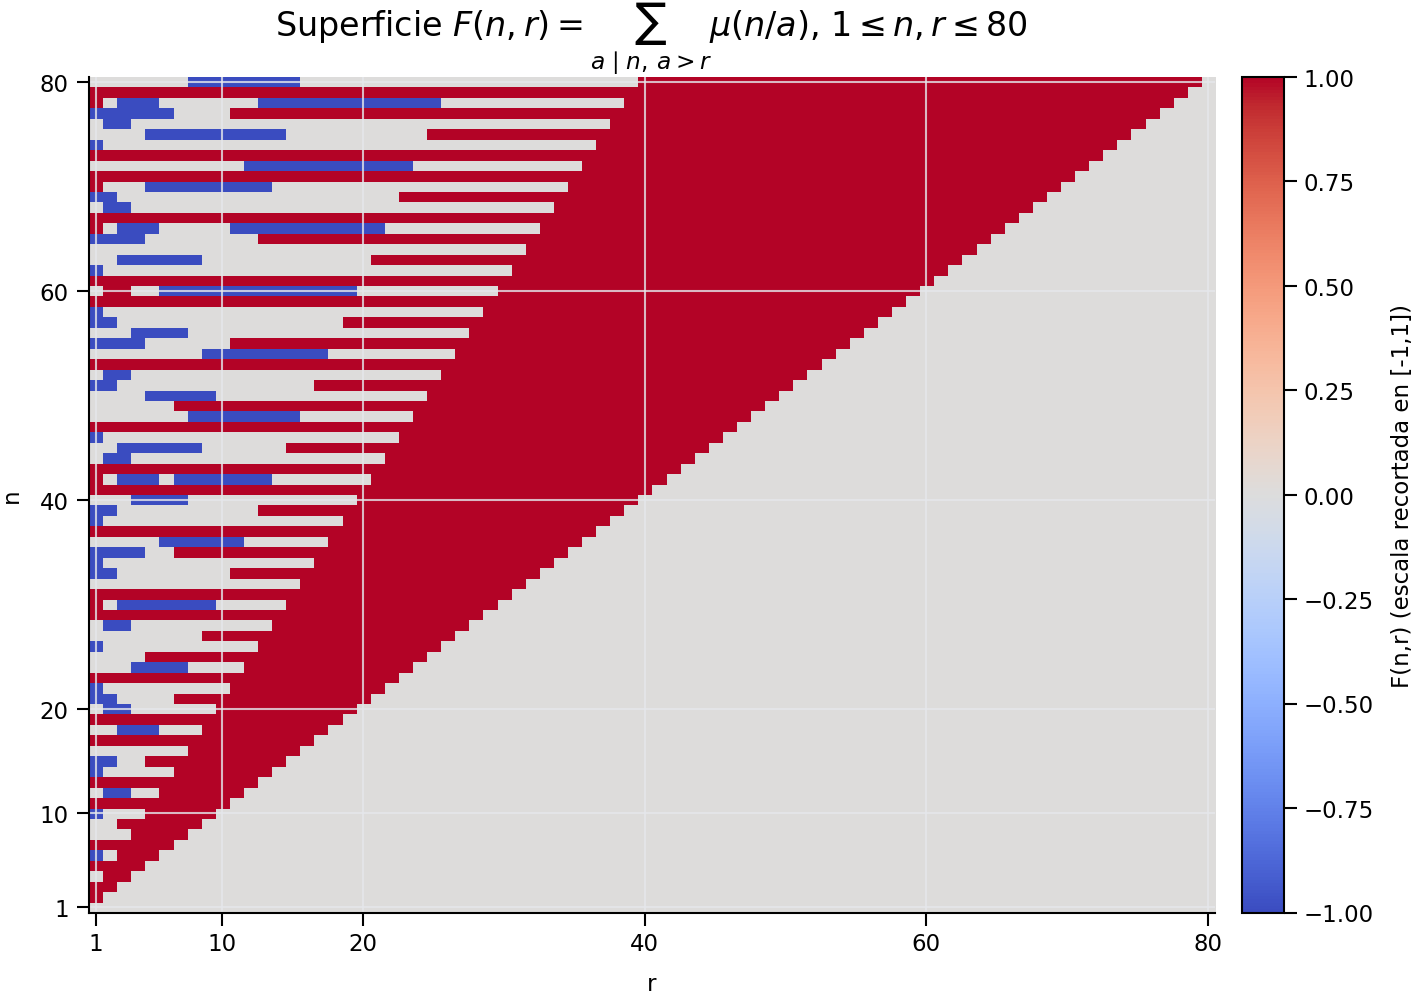
\includegraphics[width=0.92\textwidth]{mobius_heatmap_N80.png}
\caption{Heatmap of the surface \(\Fsurf(n,r)=\sum_{a\mid n,\,a>r}\mob(n/a)\), clipped to the color interval \([-1,1]\), for \(1\le n,r\le80\).  The triangular support reflects \(\Fsurf(n,r)=0\) for \(r\ge n\).}
\label{fig:heatmap}
\end{figure}

\begin{figure}[htbp]
\centering
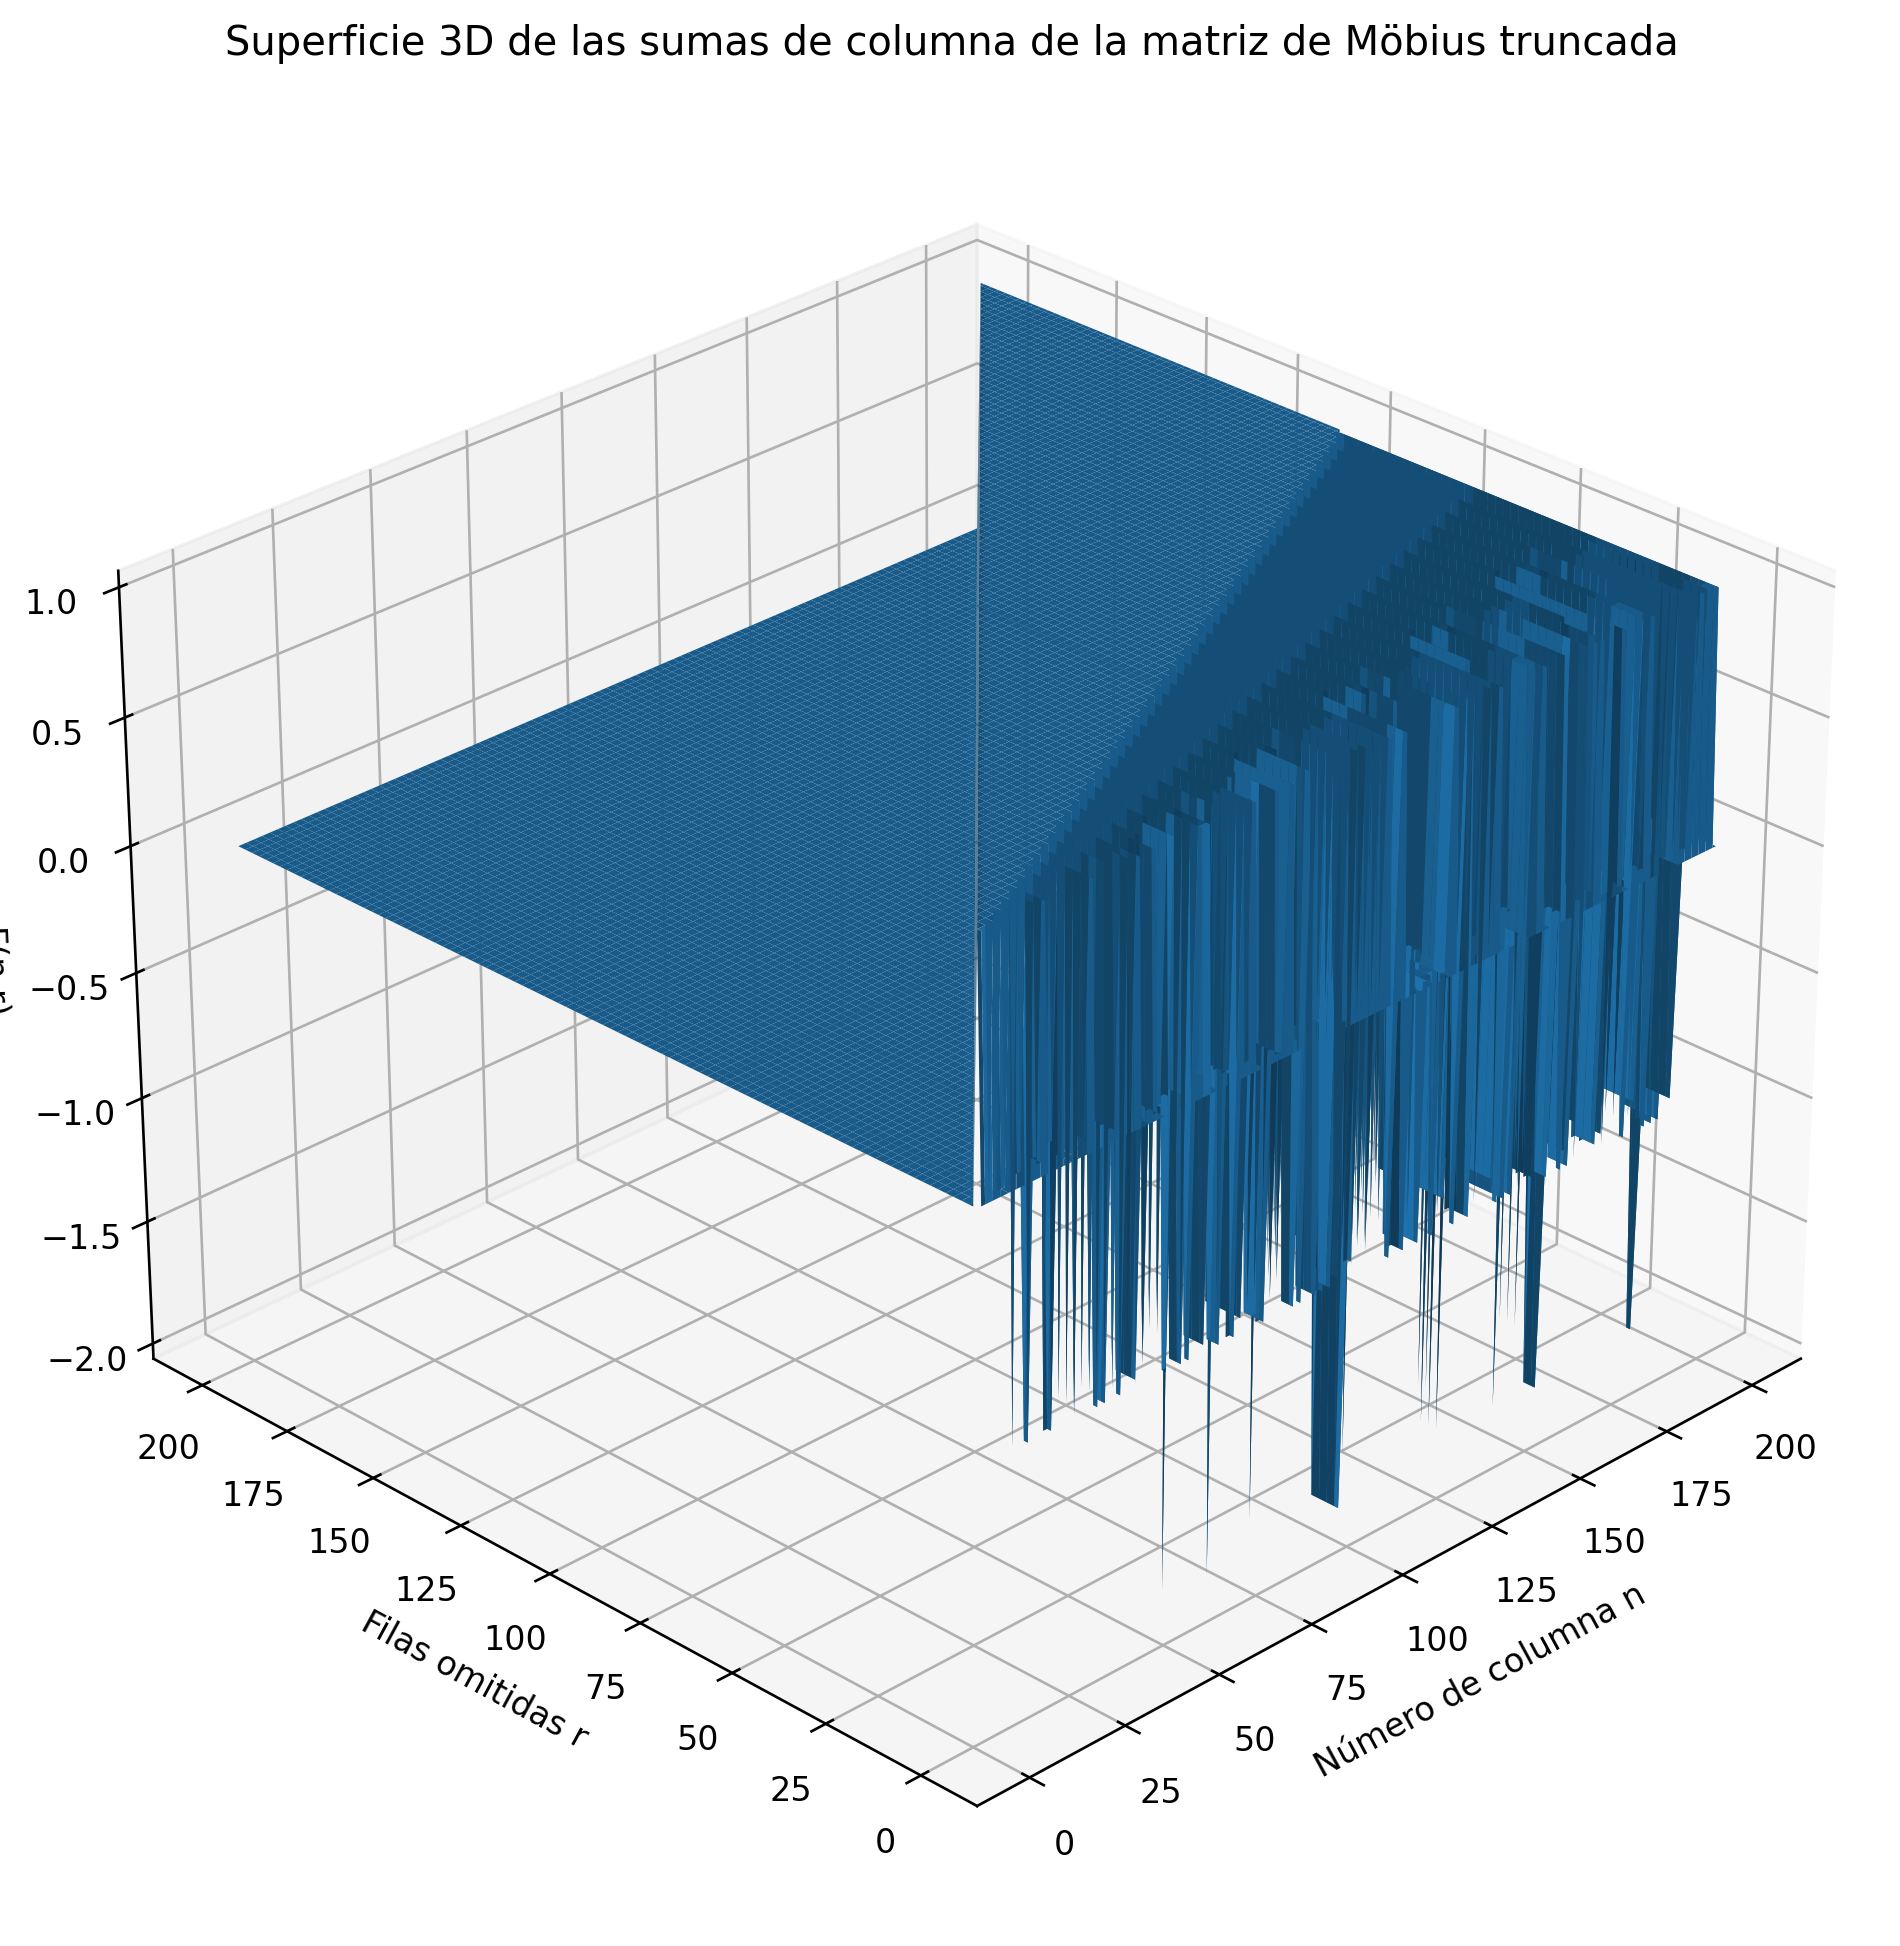
\includegraphics[width=0.92\textwidth]{mobius_surface_3d_N200.png}
\caption{Three-dimensional visualization of \(\Fsurf(n,r)\) for \(1\le n\le200\) and \(0\le r\le200\).  The plot is illustrative only; all theorems in the paper are finite algebraic identities or explicitly stated external consequences.}
\label{fig:surface3d}
\end{figure}

\section{Conclusion and next theorem to prove}
\label{sec:conclusion}

The finite part of the construction is rigorous and self-contained.  The matrix \(B_N\) is unimodular, has the explicit inverse \eqref{eq:BN_inverse}, and its inverse singular spectrum satisfies the exact identity \eqref{eq:frobenius_identity}.  The surface also intertwines ordinary first differences with Dirichlet convolution through \eqref{eq:intertwining_identity}.  These are the strongest defendable statements in this note.

The zeta quotient \(\zetaR(s+w)/\zetaR(s)\) appears naturally from the vertical jump field, but this is a classical Dirichlet-series consequence.  It should not be presented as a new route to RH.  Likewise, the Selberg diagonal rewriting \eqref{eq:Selberg_rewriting} is exact but does not improve the sieve unless row variables are treated in a genuinely multidimensional way.

The next theorem to attempt is an operator estimate for shifted row correlations.  A realistic first target is a quantitative version of Conjecture \ref{conj:operator_estimate} in a polylogarithmic range
\begin{equation}
R\le(\log X)^A,
\label{eq:next_polylog_range}
\end{equation}
with a structured main term and a power saving for the error in the weighted row norm \eqref{eq:H_norm_def}.  The ambitious target is a range \(R=X^\theta\) for some \(\theta>0\), but that should be treated as a deep program rather than a near consequence of Tao's fixed-coefficient theorem.

\begin{thebibliography}{99}

\bibitem{Apostol1976}
T. M. Apostol,
\emph{Introduction to Analytic Number Theory},
Undergraduate Texts in Mathematics, Springer, 1976.

\bibitem{BretcheDressTenenbaum2020}
R. de la Bret\`eche, F. Dress, and G. Tenenbaum,
Remarques sur une somme li\'ee \`a la fonction de M\"obius,
\emph{Mathematika} 66 (2020), 561--589,
doi:10.1112/mtk.12021; arXiv:1902.09956.

\bibitem{GPY2009}
D. A. Goldston, J. Pintz, and C. Y. Yildirim,
Primes in tuples I,
\emph{Annals of Mathematics} 170 (2009), 819--862,
doi:10.4007/annals.2009.170.819.

\bibitem{HelfgottRadziwill2021}
H. A. Helfgott and M. Radziwi{\l}{\l},
Expansion, divisibility and parity,
arXiv:2103.06853.

\bibitem{Maynard2015}
J. Maynard,
Small gaps between primes,
\emph{Annals of Mathematics} 181 (2015), 383--413,
doi:10.4007/annals.2015.181.1.7.

\bibitem{Mobius1832}
A. F. M\"obius,
\"Uber eine besondere Art von Umkehrung der Reihen,
\emph{Journal f\"ur die reine und angewandte Mathematik} 9 (1832), 105--123,
doi:10.1515/CRLL.1832.9.105.

\bibitem{BondarenkoSeip2015}
A. Bondarenko and K. Seip,
GCD sums and complete sets of square-free numbers,
\emph{Bulletin of the London Mathematical Society} 47 (2015), 29--41,
doi:10.1112/blms/bdu094; arXiv:1402.0249.

\bibitem{HilberdinkPushnitski2021}
T. Hilberdink and A. Pushnitski,
Spectral asymptotics for a family of LCM matrices,
arXiv:2110.14323.

\bibitem{HongLoewy2004}
S. Hong and R. Loewy,
Asymptotic behavior of eigenvalues of greatest common divisor matrices,
\emph{Glasgow Mathematical Journal} 46 (2004), 551--569,
doi:10.1017/S0017089504001807.

\bibitem{IlmonenHaukkanenMerikoski2008}
P. Ilmonen, P. Haukkanen, and J. K. Merikoski,
On eigenvalues of meet and join matrices associated with incidence functions,
\emph{Linear Algebra and its Applications} 429 (2008), 859--874,
doi:10.1016/j.laa.2008.04.026.

\bibitem{Pilatte2023}
C. Pilatte,
Improved bounds for the two-point logarithmic Chowla conjecture,
\emph{Journal of the American Mathematical Society}, published electronically 2026,
doi:10.1090/jams/1084; arXiv:2310.19357 (v2, revised December 1, 2025).

\bibitem{Redheffer1977}
R. M. Redheffer,
Eine explizit l\"osbare Optimierungsaufgabe,
\emph{Internationale Schriftenreihe Numerische Mathematik} 36 (1977), 213--216.

\bibitem{Reutenauer1993}
C. Reutenauer,
\emph{Free Lie Algebras},
London Mathematical Society Monographs, New Series 7, Oxford University Press, 1993.

\bibitem{RoblesRoy2004}
N. Robles and A. Roy,
Unexpected average values of generalized von Mangoldt functions in residue classes,
\emph{Journal of the Australian Mathematical Society} 111 (2021), 127--144,
doi:10.1017/S1446788719000715.

\bibitem{Rota1964}
G.-C. Rota,
On the foundations of combinatorial theory I. Theory of M\"obius functions,
\emph{Z. Wahrscheinlichkeitstheorie und Verw. Gebiete} 2 (1964), 340--368,
doi:10.1007/BF00531932.

\bibitem{Stanley2012}
R. P. Stanley,
\emph{Enumerative Combinatorics, Volume 1},
2nd edition, Cambridge Studies in Advanced Mathematics 49, Cambridge University Press, 2012.

\bibitem{Tao2016}
T. Tao,
The logarithmically averaged Chowla and Elliott conjectures for two-point correlations,
\emph{Forum of Mathematics, Pi} 4 (2016), e8,
doi:10.1017/fmp.2016.6; arXiv:1509.05422.

\bibitem{Titchmarsh1986}
E. C. Titchmarsh,
\emph{The Theory of the Riemann Zeta-Function},
2nd edition, revised by D. R. Heath-Brown, Oxford University Press, 1986.

\end{thebibliography}

\appendix

\section{Python code generating the figures}
\label{app:python_code}

The following script generates the heatmap, the 3D PNG, and an optional interactive HTML version of the surface.

\lstinputlisting{generate_mobius_surface_figures.py}

\end{document}
